\chapter{Groups}
\label{ch:groups}

\section{Definition and basic properties}
\label{sec:definition-and-basic-properties-grp}

\begin{definition}
    \label{def:group}
    A \emph{group} is a pair \((G, \mult)\) where \(G\) is a  set and \(\mult\)
    is a binary operation on \(G\) (i.e., a map from \(G \times G\) to \(G\))
    that satisfies the following axioms:
    \begin{enumerate}
        \item \emph{Associativity:} For all \(a, b, c \in G\), \(\mult(\mult(a,
        b), c) = \mult(a, \mult(b, c))\).
        \item \emph{Identity element:} There exists an element \(e \in G\) such
        that for all \(a \in G\), \(\mult(e, a) = \mult(a, e) = a\). This
        element is called the \emph{identity element} (or the \emph{neutral
        element}) of the group.
        \item \emph{Inverses:} For each \(a \in G\), there exists an element
        \(a\inv \in G\) such that \(\mult(a, a\inv) = \mult(a\inv, a) = e\).
    \end{enumerate}
\end{definition}

If the pair \((G, \mult)\) satisfies only the first two axioms, then it is
called a \emph{monoid}. If it satisfies only the first axiom, then it is called
a \emph{semigroup}.

We shall succumb to some abuse of language and refer to the group \((G, \mult)\)
simply as the group \(G\) when the binary operation \(\mult\) is clear from the
context. We shall also write \(ab\) or \(a \cdot b\) instead of \(\mult(a, b)\)
for the image of \((a, b)\) under the binary operation. We shall call the binary
operation `multiplication' (or more generally as the `group operation' of the
group \(G\)) and the element \(ab\) the `product' of \(a\) and \(b\). The set
\(G\) is called the `underlying set' of the group \(G\). When talking about two
groups \(G\) and \(H\), we shall often write as a subscript on \(\mult\) and
\(e\) the underlying set of the group in order to specify in which group we are
defining those terms, e.g., \(e_G\), \(\mult_H\), etc.

Because we require the existence of an identity element in a group \(G\), we can
conclude that the set \(G\) is nonempty. At the very least it must contain the
identity element. This group is called the \emph{trivial group} and is denoted
by \(\{e\}\) or simply as \(0\). Note also that any singleton \(\{*\}\) is a
group if we define the binary operation to be the trivial operation \(\mult(*,
*) = *\) so that the choice of writing \(\{e\}\) instead of \(\{*\}\) or any
other symbol is purely a matter of convention.

\begin{theorem}
    The identity element in a group is unique. For each \(a \in G\), the inverse
    element of \(a\) is unique.
\end{theorem}

\begin{proof}
    Suppose \(e\) and \(e'\) are both identity elements of a group \(G\). Then
    \[
        e = e \cdot e' = e'.
    \]
    Similarly, suppose \(b\) and \(b'\) are both inverses of \(a \in G\). Then
    \[
        b = b \cdot e = b \cdot (a \cdot b') = (b \cdot a) \cdot b' = e \cdot b' = b'.
    \]
\end{proof}

The preceding result allow us to speak of \emph{the} identity element of a group
and \emph{the} inverse of an element in a group. Thus for any element \(a\) in a
group, we can denote its inverse by \(a\inv\) without ambiguity.

% Group as a 4-tuple
It should be noted that Definition~\ref{def:group} is not the only possible
definition of a group. Since our initial definition axiomatizes the existence of
an identity element \(e\) in a group \(G\) and the existence of an inverse
\(a\inv\) for every element \(a\) in \(G\), which are unique and unique for each
\(a\in G\), respectively, it would be quite natural to present an alternative
definition that directly encodes these properties. Thus we have:
\begin{definition}
    \label{def:group-4-tuple}
    A \emph{group} is a 4-tuple \((G, \mult, \iota, e)\) where \(G\) is a set,
    \(\mult\) is a binary operation on \(G\), \(\iota\) is a map \(G \to G\) and
    \(e\) is an element of \(G\) such that:
    \begin{enumerate}[label=(\alph*), itemsep=0pt]
        \item For all \(a, b, c \in G\), \(\mult(\mult(a, b), c) = \mult(a,
        \mult(b, c))\).
        \item For all \(a \in G\), \(\mult(a, e) = \mult(e, a) = a\).
        \item For all \(a \in G\), \(\mult(a, \iota(a)) = \mult(\iota(a), a) =
        e\).
    \end{enumerate}
\end{definition}

Observe that one major difference between the two definitions is that the second
definition explicitly posits the existence of a map \(\iota: G \to G\) which
then reduces each of the axioms to universal statements for all elements of
\(G\). While this point might seem pedantic, such a definition is often useful
especially in the context of universal algebra where one would want to look at
more general algebraic structures (see e.g., Bergman). Still, the equivalence of
the two definitions can be immediately deduced. In particular if we define
\(\iota\) as the map \(a \mapsto a\inv\) (where \(a\inv\) is the unique inverse
of \(a\) based on Definition~\ref{def:group}), then this satisfies property (c)
of Definition~\ref{def:group-4-tuple}, viz.,
\[
    \mult(a, a\inv) = \mult(a\inv, a) = e.
\]
Nonetheless, we shall content ourselves with Definition~\ref{def:group} for the
remainder of these notes.

To further illustrate this definition, consider a group \((G, \mult, \iota,
e)\). Write \(\mult(a,b)\) as \(a\cdot b\) and suppose \(\delta : G \to G\) is a
map such that for all \(a, b \in G\),
\[
    \delta(a, b) = a\cdot\iota(b).
\]
Does \((G, \delta)\) determine the group \((G, \mult, \iota, e)\)? That is if
\((G, \mult, \iota, e)\) and \((G', \mult', \iota', e')\) yield the same pair
\((G, \delta') = (G', \delta')\), then must
\[(G, \mult, \iota, e) = (G', \mult', \iota', e')?\]

Let \((G', \mu', \iota', e')\) be another group and let \((G', \delta')\) be
similarly defined. Now suppose \((G, \delta) = (G' \delta')\), i.e., \(G = G'\)
and for all \(a, b \in G = G'\) we have
\[
\delta(a, b) = a \cdot \iota(b) = a * \iota'(b) = \delta'(a, b).
\]
where \(\mu(a, b) = a \cdot b\) and \(\mu'(a', b') = a' * b'\).

Now observe that
\[
e = a \cdot \iota(a) = \delta(a, a) = \delta'(a, a) = a * \iota'(a) = e'.
\]
Thus the identity elements of the two groups coincide. Let \(a \in G = G'\) and
let \(\alpha = \iota(a)\) and \(\alpha' = \iota'(a)\). Then in \(G\) we have by
the equality of \(e\) and \(e'\),
\[
\iota(a) = e \cdot \iota(a) = \delta(e, a) = \delta'(e, a) = e * \iota'(a) = \iota'(a)
\]
and
\[
 \iota'(a) = e' * \iota'(a) = \delta'(e', a) = \delta(e',a) = e' \cdot \iota(a) = \iota(a).
\]
Finally, we have
\[
a \cdot b = \delta(a, \iota(b)) = \delta'(a, \iota(b)) = a * \iota'(\iota(b))
\]
but then by the equality of inverses it follows that
\[
 a * \iota'(\iota(b)) = a * \iota'(\iota'(b)) = a * b.
\]
(Here we have exploited the fact that the inverse of an inverse is the original
element, a property that will only establish in Theorem~\ref{thm:group-inverses}
below.) This shows that \((G, \mu, \iota, e) = (G', \mu', \iota', e')\). This
illustrates that the group structure is uniquely determined by the group
operation and the inverse map.

% Group as a category
We take one final excursion before studying the properties of groups in detail.
Building on the categorical intuition we have developed in
\S~\ref{sec:category-theory} of Chapter~\ref{ch:preliminaries}, we can think of
a group as a category with a single object. More explicitly, we have the
following definition.

\begin{definition}
    \label{def:group-as-category}
    A group is the \(\Hom\)-set of a groupoid with a single object.
\end{definition}

That this is equivalent to Definition~\ref{def:group} can be illustrated as
follows. Recall that a groupoid is a category in which every morphism is an
isomorphism. Let \(\catg{G}\) be a groupoid and suppose that \(*\) is the lone
object in this category. Then \(\Hom_{\catg{G}}(*, *)\) is the set of all
morphisms from \(*\) to \(*\). Because \(\catg{G}\) is a category, it admits a
composition law
\[
    \Hom_{\catg{G}}(*, *) \times \Hom_{\catg{G}}(*, *) \to \Hom_{\catg{G}}(*, *).
\]
that sends a pair of morphisms \((f, g)\) to the morphism \(f \circ g\) that is
associative, i.e., for all morphisms \(f, g, h \in \Hom_{\catg{G}}(*, *)\),
\[
    f \circ (g \circ h) = (f \circ g) \circ h.
\]
and admits an identity morphism \(\id_{*}\) such that for all morphisms \(f\),
\[
    f \circ \id_{*} = f = \id_{*} \circ f.
\]
Since every morphism in \(\catg{G}\) is an isomorphism, each morphism \(f\) in
this category has an inverse \(f\inv\) such that
\[
    f \circ f\inv = \id_{*} = f\inv \circ f.
\]
Moreover, this inverse is unique
(Theorem~\ref{thm:isomorphism-unique-inverse-category},
Ch.~\ref{ch:preliminaries}). Taking these properties together, we observe that
the elements of the set \(\Hom_{\catg{G}}(*, *)\) satisfy the axioms of a group.
Thus a group can be thought of as the set of morphisms in a groupoid with a
single object.

\begin{theorem}
    \label{thm:group-inverses}
    Let \(G\) be a group and let \(a \in G\). Then \((a\inv)\inv = a\). If in
    addition, \(b \in G\), then \((ab)\inv = b\inv a\inv\).
\end{theorem}

\begin{proof}
    Suppose \(b \neq a\) is the inverse of \(a\inv\) where \(b \in G\). Then
    \(a\inv b = e = ba\inv\). But \(a\) also satisfies this property, and since
    inverses are unique, we must have \(b = a\).

    On the other hand we have
    \[
        (ab)(b\inv a\inv) = a(bb\inv)a\inv = aea\inv = aa\inv = e.
    \]
\end{proof}


\begin{theorem}[Cancellation laws]
    Let \(G\) be a group. For all \(a, b, c \in G\),
    \begin{enumerate}
        \item If \(ab = ac\), then \(b = c\).
        \item If \(ba = ca\), then \(b = c\).
    \end{enumerate}
\end{theorem}

\begin{proof}
    We prove the first statement. Suppose \(ab = ac\). Then
    \begin{align*}
        a\inv(ab) &= a\inv(ac) &\\
        (a\inv a)b &= (a\inv a)c &\text{(associativity)}\\
        eb &= ec &\text{(definition of inverse)}\\
        b &= c. &\text{(definition of identity)}
    \end{align*}
    The second statement is proved similarly.
\end{proof}

\begin{corollary}
    For all \(a, b \in G\), the equations \(ax = b\) and \(ya = b\) have unique
    solutions in \(G\).
\end{corollary}

\begin{proof}
    Observe that the solutions to the equations are \(x = a\inv b\) and \(y =
    ba\inv\), respectively. In the first case we have
    \[
        ax = a(a\inv b) = (aa\inv)b = eb = b.
    \]
    If \(x'\) is also a solution for the first equation then \(xa = b = x'a\)
    implies \(x = x'\) by right cancellation. The second equation is proved
    similarly.
\end{proof}

\begin{theorem}[Generalized associative law]
    \label{thm:generalized-associative-law}
    Let \(G\) be a group and let \(a_1, a_2, \ldots, a_n\) be elements of \(G\).
    Then the product \(a_1 a_2 \cdots a_n\) is well-defined, i.e., it is
    independent of the way in which the product is bracketed.
\end{theorem}

\begin{proof}
    We prove this by induction on \(n\). The case \(n = 2\) is the associative
    axiom in our definition of a group. If \(n > 2\), then from the definition
    of associativity
    \[
        a_1 a_2 \cdots a_n = (a_1 a_2 \cdots a_m)(a_{m + 1} \cdots a_n)
    \]
    for some \(m < n\). By induction we then have
    \begin{align*}
        a_1 a_2 \cdots a_n & = \left(\prod_{i = 1}^m a_i\right)\left(\prod_{i = 1}^{n - m} a_{m + i}\right)\\
        & = \left(\prod_{i =1}^{m}\right)\left(\left(\prod_{i = 1}^{n - m - 1} a_{m + i}\right)a_n\right)\\
        & = \left(\left(\prod_{i = 1}^{m}\right)\left(\prod_{i = 1}^{n - m- 1} a_{m + i}\right)\right)a_n\\
        & = \left(\prod_{i = 1}^{n - 1} a_i\right)a_n.
    \end{align*}
\end{proof}

\begin{remark}
    Theorem \ref{thm:generalized-associative-law} tells us that we can write
    \(a_1 a_2 \cdots a_n\) as a meaningful product without the need for
    brackets. Where each of the \(a_i\) is equal to an element \(a\) of the
    group, we shall write \(a^n\) for the product of \(n\) terms of \(a\). Thus
    \(a^1 = a\), \(a^2 = aa\), and so on. We also define \(a^0\) to be the
    identity element of the group and \(a^{-n}\) to be \((a\inv)^n\).
\end{remark}

\begin{theorem}
    If \(G\) is a group and \(a \in G\), then for all integers \(m, n\),
    \begin{enumerate}[label=(\alph*)]
        \item \((a^n)\inv = (a\inv)^n\),
        \item \(a^m a^n = a^{m + n}\), and
        \item \((a^m)^n = a^{mn}\).
    \end{enumerate}
\end{theorem}

\begin{proof}
    We prove each part in turn.
    \begin{enumerate}[label=(\alph*), wide]
        \item We prove this by induction on \(n\). The case \(n = 1\) is
        trivial. Suppose the result holds for \(n = k\). Then
        \begin{align*}
            a^{k + 1} & = a^k a\\
            (a^{k + 1})\inv & = (a^k a)\inv = a\inv (a^k)\inv\\
            & = a\inv (a\inv)^k = (a\inv)^{k + 1}.
        \end{align*}
        \item We only outline the proof. For \(m > 0\), \(n > 0\) this result
        follows directly from the generalized associative law. For \(m < 0\),
        \(n < 0\), we can replace \(a, m, n\) by \(a\inv, -m, -n\) respectively
        and argue similarly. The case \(m = 0\) and \(n = 0\) is trivial. The
        case \(m \geq 0\), \(n < 0\) and \(m < 0\), \(n \geq 0\) can be shown by
        induction on \(m\) and \(n\), respectively.
        
        \item TODO

    \end{enumerate}
\end{proof}


\begin{definition}
    A group \(G\) is said to be \emph{abelian} (or \emph{commutative}) if for
    all \(a, b \in G\),
    \[
        ab = ba.
    \]
\end{definition}

As a matter of convention, we shall write \(a + b\) instead of \(ab\) in an
abelian group and refer to the operation and the term \(a + b\) as `addition'
and the `sum' of \(a\) and \(b\), respectively. We shall also write \(-a\)
instead of \(a\inv\), \(na\) instead of \(a^n\), and \(0\) for the identity
element of the group. The sum \(a + (-b)\) for elements \(a, b\) of an abelian
group will also be abbreviated to \(a - b\). Note that \(na\) does not refer to
the `group product' in the sense of our definition of a group, but is purely a
matter of notation. (Indeed such a `product' might not even make sense given
that \(n\) is not necessarily an element of the group.)

\begin{theorem}
    In an abelian group \(G\), \((ab)^n = a^n b^n\) and \((ab)\inv = a\inv
    b\inv\) for all \(a, b \in G\) and all integers \(n\).
\end{theorem}

\begin{proof}
    We prove the first statement by induction on \(n\). The case \(n = 1\) is
    trivial. Suppose the result holds for \(n = k\). Then
    \[
        (ab)^{k + 1} = (ab)^k ab = a^k b^k ab = a^k a b^k b = a^{k + 1} b^{k + 1}.
    \]
    On the other hand, we have
    \[
        (ab)(a\inv b\inv) = a(ba\inv)b\inv = a(a\inv b)b\inv = e
    \]
    and
    \[
        (a\inv b\inv)(ab) = a\inv(b\inv a)b = a\inv(a b\inv)b = e.
    \]
\end{proof}

\begin{definition}
    An element \(a\) of a group \(G\) is said to have \emph{finite order} if
    there exists a positive integer \(n\) such that \(a^n = e\). In this case,
    the smallest such positive integer is called the \emph{order} of \(a\) and
    is denoted by \(\order{a}\). If no such positive integer exists, then \(a\)
    is said to have \emph{infinite order} and we write \(\order{a} = \infty\).
\end{definition}

We make the following analogous definition for a group \(G\):

\begin{definition}
    The order of a group \(G\) is the cardinality of the undelrying set \(G\),
    denoted by \(\order{G}\). If \(\order{G}\) is finite, then \(G\) is said to
    be a group of \emph{finite order}. Otherwise, \(G\) is said to be a group of
    \emph{infinite order} and we write \(\order{G} = \infty\).
\end{definition}

\begin{theorem}
    If \(g^n = e\) for some integer \(n\), then \(\order{g}\) divides \(n\).
\end{theorem}

\begin{proof}
    From the definition of order, we immediately have \(n \geq \order{g}\). Let
    \(\nu = \order{g}\). Then by the division algorithm, we can write \(n = q\nu
    + r\) for some integers \(q\) and \(r\) with \(0 \leq r < \nu\). Then
    \[
        e = g^n = g^{q\nu + r} = (g^\nu)^q g^r = e^q g^r = g^r.
    \]
    Thus \(r = 0\) and \(n = q\nu\) and thus \(\nu = \order{g}\) divides \(n\).
\end{proof}

\section{Examples of groups}
\label{sec:examples-of-groups}

\begin{example}[Symmetric groups]
    \label{ex:symmetric-group}
    Let \(X\) be a set. The set of all bijections from \(X\) to itself forms a
    group under composition of functions, called the \emph{symmetric group} (or
    \emph{permutation group}) on \(X\), denoted by \(\Sym{X}\). If \(X = \{1, 2,
    \ldots, n\}\), then we write \(\Symx{n}\) instead of \(\Sym{X}\). Observe
    that for any set \(X\), \(\Sym{X}\) is exactly the set of all automorphisms
    \(\Aut(X)\) in the category \(\Set\) we have defined in
    Example~\ref{ex:endomorphism-automorphism}.

    % Order of symmetric group
    What can we say about the number of elements in \(\Symx{n}\)? Since every
    element of \(\Symx{n}\) is a bijection, we can suppose that the bijection
    maps \(i\) to \(\sigma(i)\) for some \(\sigma \in \Symx{n}\). For
    \(\sigma(1)\), there are \(n\) possible choices since it can be mapped to
    any element of \(X\). With \(\sigma(1)\) fixed, there remain \(n-1\) choices
    for \(\sigma(2)\), and so on. Continuing in this manner, we see that there
    are \(n(n - 1)(n - 2) \cdots 1 = n!\) elements in \(\Symx{n}\). Thus the
    order of \(\Symx{n}\) is \(n!\). This can be generalized for any set \(X\)
    of cardinality \(n\) by noting that we can do the same counting exercise for
    each \(a_i\) in \(X\).

    % Notation for symmetric group
    Since listing the rule defining the bijection would be cumbersome given how
    large the sets \(\Symx{n}\) can be (for example, a \(10\)-element set would
    have \(10! = 3,628,800\) elements), we would like to be able to permutations
    in \(\Symx{n}\) unambiguously in a shorthand manner. For the rest of this
    text we shall work with the set \({1, 2, \ldots, n}\) without loss of
    generality. Given a permutation \(\sigma \in \Symx{n}\) we write the array
    \[
        \begin{pmatrix}
            1 & 2 & \cdots & n\\
            \sigma(1) & \sigma(2) & \cdots & \sigma(n)
        \end{pmatrix}
    \]
    to mean that \(\sigma(i)\) is the image of \(i\) under \(\sigma\). If the
    images are given, we would omit the top row and write only the row of
    images. For example, given a permutation such that \(1 \mapsto 2\), \(2
    \mapsto 3\), and \(3 \mapsto 1\), we would write
    \[
        \begin{pmatrix}
            1 & 2 & 3\\
            2 & 3 & 1
        \end{pmatrix},
    \]
    or simply \((2\ 3\ 1)\).

    This is not the most efficient way to write permutations; one would often
    encounter `cycle notation' when dealing with permutations. For our purposes,
    however, the shorthand we have introduced will suffice.

    Now on to proving that \(\Symx{n}\) is a group. We first note that the
    identity element of \(\Symx{n}\) is the identity function on \(X\) (this
    follows directly from permutations being bijections on \(X\), with the
    uniqueness following similarly). The inverse of a permutation \(\sigma\) is
    the permutation that undoes the action of \(\sigma\), i.e., the inverse
    function \(\sigma^{-1}\): again this is unique and well-defined because
    \(\sigma\) is a bijection. Finally, the associativity of permutations
    follows from the associativity of function composition.
\end{example}

\begin{example}[Dihedral groups]
    Consider an equilateral triangle in the plane with vertices \(A\), \(B\),
    and \(C\). Let \(\alpha_X\) be the line segment that joins the vertex \(X\)
    to the midpoint of the opposite side (because the triangle is equilateral,
    this line segment is perpendicular to the side opposite \(X\) and bisects
    both the side opposite \(X\) and the angle at \(X\)). We call \(\alpha_X\)
    the \emph{axis of symmetry} of the triangle with respect to the vertex
    \(X\). The axes of symmetry for each of the vertices of the \(A\), \(B\),
    and \(C\) intersects at some point in \(c\) in the interior of the triangle;
    call this point the \emph{center} of the triangle. Graphically, the
    situation is as follows:
    \begin{center}
        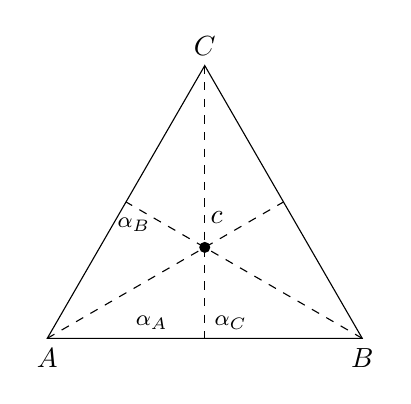
\begin{tikzpicture}
            \coordinate (A) at (0, 0); \coordinate (B) at (4, 0); \coordinate
            (C) at (2, 3.464); \draw (A) -- (B) -- (C) -- cycle;
            % dashed lines
            \draw[dashed] (C) -- (2, 0); \draw[dashed] (A) -- (3, 1.732);
            \draw[dashed] (B) -- (1, 1.732);

            % labels
            \node[below] at (A) {\(A\)}; \node[below] at (B) {\(B\)};
            \node[above] at (C) {\(C\)}; \node[right] at (2, 0.2)
            {{\footnotesize \(\alpha_C\)}}; \node[right] at (1, 0.2)
            {{\footnotesize \(\alpha_A\)}}; \node[below] at (1.1, 1.65)
            {{\footnotesize \(\alpha_B\)}};

            % center
            \node[below] at (2.15, 1.732) {\(c\)};
            % Filled circle at center
            \fill (2, 1.155) circle (2pt);

        \end{tikzpicture}
    \end{center}

    We define a rotation of the triangle \(ABC\) as a rotation of the plane
    about the center \(c\) that maps the triangle to itself (with the vertices
    permuted). For this to make sense, the rotation must be by a multiple of
    \(2\pi/3\) radians (since a circle has \(2\pi\) radians and the triangle is
    equilateral); otherwise the resulting triangle would not coincide with the
    original. To simplify, suppose \(r\) is the counterclockwise rotation by
    \(2\pi/3\) radians. Then \(r\) will map the vertex \(A\) to \(B\), \(B\) to
    \(C\), and \(C\) to \(A\). The composition \(r \circ r\) is again another
    rotation, sending the original vertex \(A\) to \(C\) and so forth; finally
    \(r \circ r \circ r\) is the identity rotation will map each vertex to
    itself. Thus we need only consider the three unique rotations \(r\), \(r
    \circ r\), and \(r \circ r \circ r\), which we thus denote \(r_1\), \(r_2\),
    and \(r_0\), respectively.

    On the other hand, we define a reflection of the triangle \(ABC\) as a
    reflection of the plane about one of the axes of symmetry of the triangle.
    For example, the reflection about the axis of symmetry \(\alpha_A\) will map
    the vertex \(A\) to itself, \(B\) to \(C\), and \(C\) to \(B\). The
    composition of two reflections is again a reflection, and the composition of
    the same reflection about the same axis of symmetry results in the original
    triangle. Thus we need only consider the three unique reflections about the
    axes of symmetry \(\alpha_A\), \(\alpha_B\), and \(\alpha_C\), which we
    denote \(s_A\), \(s_B\), and \(s_C\), respectively.

    The actions defined by \(s_X\) and \(r_i\) interact with each other in a
    regular way. For example, if we reflect the triangle about the axis of
    symmetry \(\alpha_A\) and then rotate the triangle by \(2\pi/3\) radians
    counterclockwise, we obtain the same result by just reflecting the triangle
    about the axis of symmetry \(\alpha_C\), that is, the composition
    \begin{center}
        \begin{tikzpicture}
            \coordinate (A) at (0, 0); \coordinate (B) at (2, 0); \coordinate
            (C) at (1, 1.732); \draw (A) -- (B) -- (C) -- cycle;
            % labels
            \node[below] at (A) {\(A\)}; \node[below] at (B) {\(B\)};
            \node[above] at (C) {\(C\)};

            % node mapsto
            \node at (3, 0.866) {\(\overset{s_A}{\mapsto}\)};
        \end{tikzpicture}
        \begin{tikzpicture}
            \coordinate (A) at (0, 0); \coordinate (B) at (2, 0); \coordinate
            (C) at (1, 1.732); \draw (A) -- (B) -- (C) -- cycle;
            % labels
            \node[below] at (A) {\(A\)}; \node[below] at (B) {\(C\)};
            \node[above] at (C) {\(B\)};

            % node mapsto
            \node at (3, 0.866) {\(\overset{r_1}{\mapsto}\)};
        \end{tikzpicture}
        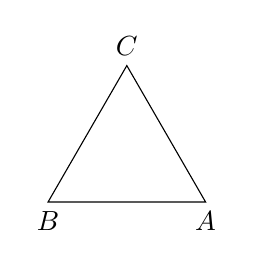
\begin{tikzpicture}
            \coordinate (A) at (0, 0); \coordinate (B) at (2, 0); \coordinate
            (C) at (1, 1.732); \draw (A) -- (B) -- (C) -- cycle;
            % labels
            \node[below] at (A) {\(B\)}; \node[below] at (B) {\(A\)};
            \node[above] at (C) {\(C\)};
        \end{tikzpicture}
    \end{center}
    is the same as
    \begin{center}
        \begin{tikzpicture}
            \coordinate (A) at (0, 0); \coordinate (B) at (2, 0); \coordinate
            (C) at (1, 1.732); \draw (A) -- (B) -- (C) -- cycle;
            % labels
            \node[below] at (A) {\(A\)}; \node[below] at (B) {\(B\)};
            \node[above] at (C) {\(C\)};

            % node mapsto
            \node at (3, 0.866) {\(\overset{s_C}{\mapsto}\)};
        \end{tikzpicture}
        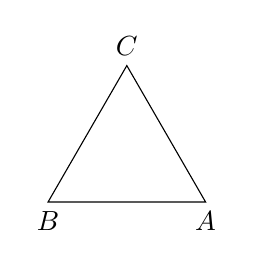
\begin{tikzpicture}
            \coordinate (A) at (0, 0); \coordinate (B) at (2, 0); \coordinate
            (C) at (1, 1.732); \draw (A) -- (B) -- (C) -- cycle;
            % labels
            \node[below] at (A) {\(B\)}; \node[below] at (B) {\(A\)};
            \node[above] at (C) {\(C\)};
        \end{tikzpicture}
    \end{center}
    In particular, a routine verification will establish the following
    identities:
    \[
        r_2 = r_1 \circ r_1, \quad s_B = s_A \circ r_1 \circ r_1, \quad s_C = s_A \circ r_1.
    \]

    Writing \(r\) for \(r_1\) and \(s\) for \(s_A\) and using the exponential
    notation we have introduced in
    \S~\ref{sec:definition-and-basic-properties-grp}, the distinct elements of
    \(D_3\) are then
    \[
        D_3 = \{e = r_0, r, r^2, r, rs, r^2s\}.
    \]
    Here we write \(rs\) to mean the composition of the rotation \(r\) and the
    reflection \(s\), i.e., \(rs = s\circ r\). We can more succinctly write
    these identities using the following commutative diagram, where each arrow
    represents the rotation \(r\) and each dashed arrow represents the
    reflection \(s\):
    \begin{center}
        \begin{tikzpicture}[ vertex/.style={circle, draw=black, minimum
            size=0.85cm}, edge/.style={->, >=Stealth, thick},
            double/.style={<->, >=Stealth, thick},every
            node/.style={font=\small} ]
        
        % Define vertices
        \node[vertex] (e) at (0, 0) {\scriptsize\(e\)}; \node[vertex] (r) at (2,
        0) {\scriptsize\(r\)}; \node[vertex] (r2) at (1, 1.732)
        {\scriptsize\(r^2\)};
        
        % Extend the triangle by making another equilateral triangle containing
        % the first
        \draw[edge] (e) -- (r); \draw[edge] (r) -- (r2); \draw[edge] (r2) --
        (e); \node[vertex] (s) at (-1.6, -1.3) {\scriptsize\(s\)}; \node[vertex]
        (sr) at (3.6, -1.3) {\scriptsize\(rs\)};
        % sqrt(2) = 1.414 * 3 = 4.242/2 = 2.121 + 1.732 = 3.853
        \node[vertex] (sr2) at (1, 3.853) {\scriptsize\(r^2s\)}; \draw[double,
        dashed] (e) -- (s); \draw[double, dashed] (r) -- (sr); \draw[double,
        dashed] (r2) -- (sr2); \draw[edge] (sr) to [bend left=20] (s);
        \draw[edge] (sr2) to [bend left=20] (sr); \draw[edge] (s) to [bend
        left=20] (sr2);
        \end{tikzpicture}
    \end{center}
    This is called the Cayley diagram of the group \(D_3\). In particular, the
    Cayley diagram of \(D_3\) shows that the choice of the initial configuration
    of the vertices of the triangle is irrelevant. Since the relations between
    the elements of \(D_3\) are preserved regardless of the chosen starting
    configuration (because we have defined \(e\) to be exactly the identity map
    that leaves the triangle unchanged), we can ignore the specific arrangement
    of the vertices and focus solely on the elements and structure of \(D_3\).

    With our notation fixed, we observe that \(e \tau = \tau  e = \tau\) for all
    maps \(\tau \in D_3\). Moreover, any composition of elements of \(D_3\) is
    again an element of \(D_3\) and this composition is likewise associative.
    Similarly, the commutativity of the Cayley diagram and the fact that the
    elements of \(D_3\) exhausts all possible unique configurations of the
    triangle in consideration (by our definition) tell us that \(\tau \in R\)
    has an inverse in \(R\): that is, given any node \(\tau\) in the Cayley
    diagram, there is a finite sequence of arrows (which can either be a
    reflection or a rotation) that will take us back to the identity element
    \(e\), thus undoing the action of \(\tau\), and because all possible
    configurations of \(D_3\) are expressible as one of the nodes of the Cayley
    diagram, this sequence must then be the same as one of the elements of
    \(D_3\). We can immediately verify, for example, that the inverse of a
    reflection is the reflection about the same axis of symmetry. Similarly, the
    inverse of a rotation is a rotation in the opposite direction; however,
    since a rotation in the opposite direction is not well-defined (as we have
    only defined rotations in one direction), we can instead consider the fact
    that a rotation followed by two subsequent rotations in the same direction
    brings us back to the identity element, and thus \(r = r^2\). For a less
    trivial example, consider the element \(r^2s\) in the Cayley diagram;
    observe that \(r^2s \overset{s}{\mapsto} r^2 \overset{r}{\mapsto} e\), and
    thus \((r^2s)\inv = sr\), but then \(e \overset{s}{\mapsto} s
    \overset{r}{\mapsto} r^2s\), and therefore \((r^2s)\inv = r^2s\). Indeed the
    path \(r^2s \overset{r}{\mapsto} rs \overset{r}{\mapsto} s
    \overset{s}{\mapsto} e\) shows that \(r^2s\) is its own inverse. Thus
    \(D_3\) is a group under composition of functions. We call \(D_3\) the
    \emph{dihedral group} of order \(6\), the group of symmetries of a regular
    triangle. 

    We can extend our definition to regular \(n\)-gons for arbitrary \(n \geq
    3\). Each group \(D_n\) would have \(n\) rotations (defined by rotating the
    plane about its center by \(2\pi/n\) radians) and \(n\) reflections (defined
    by reflecting the plane about the axes of symmetry for each of the \(n\)
    vertices). The group \(D_n\) is thus a group of order \(2n\).\footnote{An
    alternative notation is to write \(D_n\) as \(D_{2n}\) to emphasize the
    order of the group. This is more common in algebra texts, with \(D_n\)
    preferred in geometry.} For example, the group \(D_4\) would have \(8\)
    elements and is given by the following Cayley diagram:
    \begin{center}
        \begin{tikzpicture}[ vertex/.style={circle, draw=black, minimum
            size=0.85cm}, edge/.style={->, >=Stealth, thick},
            double/.style={<->, >=Stealth, thick}, every
            node/.style={font=\small} ]
        
        % Define vertices
        \node[vertex] (e) at (0, 0) {\scriptsize\(e\)}; \node[vertex] (r) at (2,
        0) {\scriptsize\(r\)}; \node[vertex] (r2) at (2, 2)
        {\scriptsize\(r^2\)}; \node[vertex] (r3) at (0, 2) {\scriptsize\(r^3\)};
        
        % Extend the triangle by making another equilateral triangle containing
        % the first
        \draw[edge] (e) -- (r); \draw[edge] (r) -- (r2); \draw[edge] (r2) --
        (r3); \draw[edge] (r3) -- (e); \node[vertex] (s) at (-1.6, -1.3)
        {\scriptsize\(s\)}; \node[vertex] (sr) at (3.6, -1.3)
        {\scriptsize\(rs\)}; \node[vertex] (sr2) at (3.6, 3.3)
        {\scriptsize\(r^2s\)}; \node[vertex] (sr3) at (-1.6, 3.3)
        {\scriptsize\(r^3s\)}; \draw[double, dashed] (e) -- (s); \draw[double,
        dashed] (r) -- (sr); \draw[double, dashed] (r2) -- (sr2); \draw[double,
        dashed] (r3) -- (sr3); \draw[edge] (sr) -- (s); \draw[edge] (sr2) --
        (sr); \draw[edge] (sr3) -- (sr2); \draw[edge] (s) -- (sr3);
        \end{tikzpicture}
    \end{center}
    Remembering all the relationships between the elements of \(D_n\) is
    cumbersome (and might appear even arbitrary at a glance) but we need only
    note that since the arrows are either reflections or rotations, we can fully
    express them in terms of \(r\) and \(s\). In particular, in \(D_3\), we have
    \[
        r^3 = e, \quad s^2 = e, \quad rsrs = e.
    \]
    The relations can be verified by looking at the Cayley diagram of \(D_3\)
    but the proof that these and these relations alone uniquely determines
    \(D_3\) relies on the notion of a free group and the first isomorphism
    theorem, which we discuss in~\S~\ref{sec:quotient-groups}.

    As a final note, observe that if we fix the position of \(A\) and write
    \((ABC)\) for this configuration, each element of \(D_3\) then determines a
    permutation of the vertices of the triangle, and thus we can define a map
    from \(D_3\) to \(\Symx{3}\). We will explore this again once we have
    defined the notion of a homomorphism.
\end{example}

\begin{example}[Linear groups]
    \label{ex:linear-groups}
    The \emph{general linear group} of dimension \(n\), \(\GL_n(\mathsf{k})\) is
    the group of all invertible \(n \times n\) matrices with entries in a field
    \(\mathsf{k}\) under matrix multiplication. We verify that
    \(\GL_n(\mathsf{k})\) is a group, relying on results from linear algebra
    which we shall not explore in detail presently. Since invertible matrices
    have nonzero determinants, for any two matrices \(A, B \in
    \GL_n(\mathsf{k})\), \(\det(AB) = \det(A)\det(B) \neq 0\), and thus \(AB\)
    is invertible. The identity matrix is the identity element of
    \(\GL_n(\mathsf{k})\), and the inverse of a matrix is its inverse in the
    usual sense of matrix algebra. The associativity of matrix multiplication
    follows from the associativity of multiplication in the field
    \(\mathsf{k}\). Observe that \(\GL_n(\mathsf{k})\) is not abelian for \(n >
    1\), as matrix multiplication is not commutative in general.

    The \emph{special linear group} of dimension \(n\), \(\SL_n(\mathsf{k})\)
    consists of all matrices in \(\GL_n(\mathsf{k})\) with determinant \(1\).
    The group operation as well as inverses are similarly defined. The identity
    matrix \(I_n\) has determinant \(1\) and must therefore be in
    \(\SL_n(\mathsf{k})\). More generally, for \(\SL_n(\mathsf{k})\), we require
    only that \(\mathsf{k}\) be a commutative ring \(R\) with unity, not
    necessarily a field.
\end{example}

\begin{example}[\(\Z\) and \(\Z/n\Z\)]
    \label{def:z-and-zmodn}
    The set of integers \(\Z\) forms a group under the usual addition of
    integers with identity element \(0\). Let \(n\) be a positive integer.
    Recall that congruence modulo \(n\), defined by
    \[
        a \equiv b \pmod{n} \quad \text{if and only if} \quad n \mid (a - b),
    \]
    for all integers \(a, b\), is an equivalence relation on \(\Z\). We define
    \(\Z/n\Z\) to be the set of equivalence classes of this relation. We can
    verify that \(\Z/n\Z\) consists of exactly \(n\) elements, namely
    \[
        [0]_n, [1]_n, \ldots, [n - 1]_n,
    \]
    where \([a]_n\) denotes the equivalence class of \(a\) modulo \(n\). We
    define the group operation on \(\Z/n\Z\) by
    \[
        [a]_n + [b]_n = [a + b]_n.
    \]
    which we call `addition modulo \(n\)'.  First we need to show that this
    operation is well-defined, i.e., the result of the operation does not depend
    on the choice of representatives of the equivalence classes. Suppose that
    \(a \equiv a' \pmod{n}\) and \(b \equiv b' \pmod{n}\). Then \(a = a' + kn\)
    and \(b = b' + \ell n\) for some integers \(k, \ell\). We then have
    \[
        (a' + b') - (a + b) = (a' - a) + (b' - b) = kn + \ell n = (k + \ell)n,
    \]
    and thus
    \[
        (a + b) \equiv (a' + b') \pmod{n}.
    \]
    Associativity follows from the associativity of addition in \(\Z\) and the
    identity element is \([0]_n\), viz.,
    \[
        [a]_n + [0]_n = [a + 0]_n = [a]_n.
    \]
    Similarly for each \([a]_n\) there exists an inverse \([-a]_n\) (which is
    taken to be the equivalence class of \(-a\) modulo \(n\) where \(-a\) is the
    inverse of \(a\) in \(\Z\)) such that
    \[
        [a]_n + [-a]_n = [a - a]_n = [0]_n.
    \]
\end{example}

\begin{example}[Cayley tables]
    Given a group \(G\), the \emph{Cayley table} (or \emph{multiplication
    table}) of \(G\) is a square table with \(|G|\) rows and columns where the
    entry in the \(i\)-th row and \(j\)-th column is the product of the \(i\)-th
    and \(j\)-th elements of \(G\). The Cayley table of a group is unique up to
    the order of the elements in the table. Each entry in the table is an
    element of \(G\), and each element of \(G\) appears exactly once in each row
    and column of the table: indeed, if for some fixed element \(a \in G\) such
    that \(ab = ac\), then by the cancellation law \(b = c\).
    
    The Cayley table of a group is a useful tool for understanding the structure
    of the group, especially for small groups. We would often write an outer row
    and an outer column (call them the 0th row and the 0th column for
    convenience) that list the elements of the group in some order, with the (0,
    0)th entry being the group operation. We would also often write the identity
    element in cells \(0, 1\) and \(1, 0\) so that their product (which is also
    the identity) would appear on the first row and first column.

    Consider for example the group, \(\Z/2\Z\). The Cayley table of this group
    is
    \[
        \begin{array}{c|cc}
            + & 0 & 1\\
            \hline
            0 & 0 & 1\\
            1 & 1 & 0
        \end{array}
    \]

    We can illustrate the usefulness of Cayley tables by considering groups of
    order up to \(3\). We claim that there is only one way to construct a Cayley
    table for groups of order \(1\), \(2\), and \(3\). The case \(|G| = 1\) is
    the trivial group. If \(|G| = 2\), then it must have an identity element and
    another element \(a \neq e\). First we have \(ea = ae = a\); but what does
    \(aa\) equal? If \(aa = a\) then \(a\) is the identity element, which is a
    contradiction; since there is only one other element in the group, \(aa\)
    must equal \(e\). Thus the Cayley table of a group of order \(2\) is
    \[
        \begin{array}{c|cc}
            \cdot & e & a\\
            \hline
            e & e & a\\
            a & a & e
        \end{array}
    \]
    Observe, however, that we could have written \(e\) as \(0\) and \(a\) as
    \(1\) and obtain the Cayley table of \(\Z/2\Z\). Thus the Cayley table for a
    group of order \(2\) is unique up to some `relabelling' of its elements;
    i.e., if we know any consistent `relabelling' from \(\Z/2\Z\) to some group
    of order \(2\), then we can determine the Cayley table of that group by
    sending \(0\) to the identity element and \(1\) to the other element. There
    is a more precise way to state this result: we say that every group of order
    \(2\) is `isomorphic' to \(\Z/2\Z\). We shall define this notion more
    precisely in \S~\ref{sec:homomorphisms-grp} but shall content ourselves with
    this informal definition for now.

    Now consider a group of order \(3\). It must have an identity element \(e\)
    and two other elements, say \(a\) and \(b\), both distinct from \(e\) and
    from each other. From the definition of the identity, we have \(ea = ae =
    a\), \(eb = be = b\). Consider the product \(ab \in G\). Then \(ab\) must be
    one of \(e, a, b\) since there are only three elements in the group. If \(ab
    = b\) or \(ab = a\), then \(b = e\) or \(a = e\), respectively, which
    contradicts are assumption that both \(a\) and \(b\) are distinct from
    \(e\). Thus \(ab = e\). A similar argument shows that \(ba = e\) and \(G\)
    is abelian. Now \(aa \neq a\) because \(a\) is distinct from \(e\), and \(aa
    \neq e = ab\) because cancellation gives us \(a = b\), which is a
    contradiction. Thus \(aa = b\). Similarly, \(bb = a\). The Cayley table of a
    group of order \(3\) is then
    \[
        \begin{array}{c|ccc}
            \cdot & e & a & b\\
            \hline
            e & e & a & b\\
            a & a & b & e\\
            b & b & e & a
        \end{array}
    \]
    A similar exercise in relabelling shows that every group of order \(3\) is
    isomorphic to this group (which, by rewriting \(e\) as \(0\), \(a\) as
    \(1\), and \(b\) as \(2\), is the group \(\Z/3\Z\)).
\end{example}

\begin{example}[Cyclic groups]
    \label{ex:cyclic-group}
    A group \(C\) is said to be \emph{cyclic} if there exists an element \(g \in
    C\) such that
    \[
        C = \{g^k \mid k \in \Z\}.
    \]
    That is, every element of \(C\) is a power of \(g\). In this case, we say
    that \(C\) is \emph{generated} by \(g\), and we write \(C = \gen{g}\). If
    \(g\) has order \(n\) in \(C = \gen{g}\), then \(g^{n+1} = g\), and \(C\)
    must have a finite number of elements, namely
    \[
        C = \{e, g, g^2, \ldots, g^{n - 1}\}.
    \]
    Otherwise, if \(g\) has infinite order in \(C\), then \(C\) must likewise
    have an infinite number of elements. In the first case we call \(C\) the
    \emph{(finite) cyclic group of order \(n\)} and write \(C_n\) instead of
    just \(C\). A more common notation for the cyclic group of the infinite
    cyclic group generated by an element \(g \in C\) is \(\gen{g}\); we justify
    this notation in Example~\ref{ex:subgroup-generated-by-set}.

    It follows immediately that every cyclic group is abelian. Indeed, if \(a, b
    \in C\) (for some cyclic group \(C\)), then \(a = g^m\) and \(b = g^n\) for
    some integers \(m, n\) and
    \[
        ab = g^m g^n = g^{m + n} = g^{n + m} = g^n g^m = ba.
    \]
\end{example}

\section{Homomorphisms and the category {\normalfont\bfseries Grp}}
\label{sec:homomorphisms-grp}

Recall that we have defined a group to be the pair \((G, \mult_G)\) where \(G\)
is a set and \(\mult_G\) is a binary operation on \(G\). That is, \(\mult_G\) is
a map from \(G \times G\) to \(G\). For two groups \((G, \mult_G)\) and \((H,
\mult_H)\), we would like to define a map
\[
    \phi: (G, \mult_G) \to (H, \mult_H)
\]
that is a function (which with some abuse of notation we shall also denote by
\(\phi\)) between the underlying sets \(G\) and \(H\) that `preserves' the group
structure.

If we define the set function
\[
    \phi \times \phi: G \times G \to H \times H
\]
by
\begin{equation}
    \label{eq:phi-times-phi}
    (a, b) \mapsto (\phi(a), \phi(b))
\end{equation}
then we get the following diagram:
\begin{equation}
    \begin{tikzcd}
        G \times G \arrow{r}{\phi \times \phi} \arrow[swap]{d}{\mult_G} & H \times H \arrow{d}{\mult_H} \\
        G \arrow{r}{\phi} & H
    \end{tikzcd}
    \label{eq:group-homomorphism-diagram}
\end{equation}
Now does such a set function \(\phi \times \phi\) exist in the first place?
Recall that since \(\Set\) is a category in which products are defined, products
in \(\Set\) satisfy the universal property for products in a category, i.e.,
given the set product \(A \times B\) and the set functions \(f_A : X \to A\) and
\(f_B : X \to B\), for any set \(X\), there exists a unique set function \(f: X
\to A \times B\) such that \(f_A = \pi_A \circ f\) and \(f_B = \pi_B \circ f\),
where \(\pi_A\) and \(\pi_B\) are the projections from \(A \times B\) to \(A\)
and \(B\), respectively. 

Let \(\phi : G \to H\) be a set function and let \(\pi_{G_1}, \pi_{G_2}\) and
\(\pi_{H_1}, \pi_{H_2}\) be the projections from \(G \times G\) to \(G\) and
from \(H \times H\) to \(H\), respectively, with the subscript indicating the
component of the product to which the projection is made, i.e., \(\pi_{G_1}\)
sends \((a, b)\) to \(a\) and \(\pi_{G_2}\) sends \((a, b)\) to \(b\) for all
\(a, b \in G\). Consider now the diagram
\[
    \begin{tikzcd}
        G \arrow[r, "\phi"]                                                                  & H                                                        \\
        G\times G \arrow[d, "\pi_{G_2}"'] \arrow[u, "\pi_{G_1}"] \arrow[r, "\phi\times\phi"] & H\times H \arrow[u, "\pi_{H_1}"'] \arrow[d, "\pi_{H_2}"] \\
        G \arrow[r, "\phi"']                                                                 & H                                                       
        \end{tikzcd}
\]
First note that for all \(a, b\in G\), the composition \(\phi \circ \pi_{G_1}\)
is a function from \(G \times G\) to \(H\) that sends \((a, b)\) to \(\phi(a)\).
Similarly, \(\phi \circ \pi_{G_2}\) sends \((a, b)\) to \(\phi(b)\). The
universal property for products then tells us that there exists a unique
function \(\Phi : G \times G \to H \times H\) such that \(\phi = \pi_{H_1} \circ
\Phi\) and \(\phi = \pi_{H_2} \circ \Phi\); moreover, this function is given by 
\[
        \Phi(a, b) = (\phi\circ\pi_{G_1}(a, b), \phi\circ\pi_{G_2}(a, b))
\]
(see Example~\ref{ex:product-set-universal-property},
Ch.~\ref{ch:preliminaries}). However, by our earlier remark, this is precisely
\[
    \Phi(a, b) = (\phi(a), \phi(b))
\]
and thus the set function \(\phi \times \phi\) exists and is unique.
Furthermore, our definition in \eqref{eq:phi-times-phi} agrees with this
definition.

By requiring that the diagram in \eqref{eq:group-homomorphism-diagram} commute,
we obtain a function \(\phi: G \to H\) that does exactly what we want. Indeed if
the diagram commutes, then for all \(a, b \in G\),
\[
    \begin{tikzcd}
        (a, b) \arrow[swap, mapsto]{d}{\mult_G} & & (a, b) \arrow{r}{\phi \times \phi} & (\phi(a), \phi(b)) \arrow[mapsto]{d}{\mult_H} \\
        a\cdot b \arrow[mapsto]{r}{\phi} & \phi(a\cdot b) && \phi(a)\cdot\phi(b)
    \end{tikzcd}
\]
where \(\cdot\) on the left-hand side is the group operation in \(G\) and
\(\cdot\) on the right-hand side is the group operation in \(H\). Since the
diagram commutes, we must arrive at the same element in \(H\) by following the
two paths. This gives us the following more familiar definition.

\begin{definition}
    Let \(G\) and \(H\) be groups. A \emph{homomorphism} from \(G\) to \(H\) is
    a map \(\phi: G \to H\) that satisfies
    \[
        \phi(ab) = \phi(a)\phi(b)
    \]
    for all \(a, b \in G\).
\end{definition}

We are again being imprecise but we shall not distinguish between the the
multiplications in \(G\) and \(H\) and simply write \(\phi(ab) =
\phi(a)\phi(b)\) when the context is clear.

If \(G\) and \(H\) are groups, we denote the set of group homomorphisms from
\(G\) to \(H\) as
\[
    \Hom_{\Grp}(G, H).
\]
This allows us to define the category \(\Grp\) whose objects are groups and
whose morphisms are group homomorphisms as in the following theorem.

\begin{theorem}
    The category \(\Grp\) is a category whose objects are groups and whose
    morphisms are group homomorphisms.
\end{theorem}

\begin{proof}
    If \(G\), \(H\), and \(K\) are groups, and \(\phi: G \to H\) and \(\psi: H
    \to K\) we need to show that the composition \(\psi \circ \phi: G \to K\) is
    a group homomorphism, i.e., the following diagram commutes:
    \[
        \begin{tikzcd}
            G \times G \arrow[d, "\mult_G"] \arrow[r, "\phi \times \phi"'] \arrow[rr, "(\psi \circ \phi) \times (\psi \circ \phi)", bend left] & H\times H \arrow[d, "\mult_H"] \arrow[r, "\psi \times \psi"'] & K\times K \arrow[d, "\mult_K"] \\
            G \arrow[r, "\phi"] \arrow[rr, "\psi \circ \phi"', bend right]                                                                       & H \arrow[r, "\psi"]                                           & K                             
            \end{tikzcd}
    \]
    Because each of the inner rectangles in the diagram commutes, the outer
    rectangle must also commute. By the universal property for products, there
    must exist a unique function
    \[
        (\psi \circ \phi) \times (\psi \circ \phi): G \times G \to K \times K
    \]
    such that the diagram below commutes:
    \[
        \begin{tikzcd}
            G \arrow[rr, "\psi \circ \phi"]                                                                                &  & K                                                        \\
            G\times G \arrow[d, "\pi_{G_1}"'] \arrow[u, "\pi_{G_1}"] \arrow[rr, "(\psi \circ \phi)\times(\psi \circ\phi)"] &  & K\times K \arrow[u, "\pi_{K_1}"'] \arrow[d, "\pi_{K_2}"] \\
            G \arrow[rr, "\psi \circ \phi"']                                                                                          &  & K                                                       
            \end{tikzcd}
    \]
    On the other hand, since
    \[
            (\phi \times \phi) \circ (\psi \times \psi) : G \times G \to K \times K,
    \]
    the universal property for products again tells us that the diagram below
    commutes:
    \[
        \begin{tikzcd}
            G \arrow[r, "\phi"] \arrow[rr, "\psi \circ \phi", bend left]                         & H \arrow[r, "\psi"]                                                                  & K                                                        \\
            G\times G \arrow[d, "\pi_{G_1}"'] \arrow[u, "\pi_{G_1}"] \arrow[r, "\phi\times\phi"] & H\times H \arrow[u, "\pi_{H_1}"'] \arrow[d, "\pi_{H_2}"] \arrow[r, "\psi\times\psi"] & K\times K \arrow[u, "\pi_{K_1}"'] \arrow[d, "\pi_{K_2}"] \\
            G \arrow[r, "\phi"'] \arrow[rr, "\psi \circ \phi"', bend right]                      & H \arrow[r, "\psi"']                                                                 & K                                                       
            \end{tikzcd}
    \]
    By the uniqueness of \((\psi \circ \phi) \times (\psi \circ \phi)\) we must
    then have
    \[
        (\psi \circ \phi) \times (\psi \circ \phi) = (\phi \times \phi) \circ (\psi \times \psi).
    \]

    More explicitly, for all \(a, b \in G\),
    \begin{align*}
        (\psi \circ \phi)(ab) &= \psi(\phi(ab))&\\
        &=\psi(\phi(a)\phi(b))& (\text{since \(\phi\) is a homomorphism})\\
        &= \psi(\phi(a))\psi(\phi(b)) & (\text{since \(\psi\) is a homomorphism})\\
        &= (\psi \circ \phi)(a)(\psi \circ \phi)(b).&
    \end{align*}
    Associativity follows from the associativity of set functions (since group
    homomorphisms are set functions). For each group \(G\), the identity
    function \(\id_G: G \to G\) is a group homomorphism because for all \(a, b
    \in G\),
    \[
        \id_G(ab) = ab = \id_G(a)\id_G(b).
    \]
    Finally, this identity function is neutral with respect to composition of
    functions, i.e., for all group homomorphisms \(\phi: G \to H\),
    \[
        (\phi \circ \id_G)(a) = \phi(\id_G(a)) = \phi(a) = \id_H(\phi(a)) = (\id_H \circ \phi)(a).
    \]
    Thus \(\Grp\) is a category.
\end{proof}

It should be noted that we have defined morphisms in the category \(\Grp\) using
only the underlying set and the corresponding group operation. However, our
definition of a group also posits the existence of an identity element and of
inverses. We are able to do so because, as the following theorem shows,
preserving the group operation is enough to preserve the identity element and
inverses.

\begin{theorem}
    A homomorphism preserves the identity element and inverses, i.e., given a
    homomorphism \(\phi: G \to H\),
    \begin{enumerate}[label=(\alph*)]
        \item \(\phi(e_G) = e_H\), and
        \item \(\phi(a\inv) = \phi(a)\inv\),
    \end{enumerate}
    where \(e_G\) and \(e_H\) are the identity elements of \(G\) and \(H\)
    respectively, and \(a \in G\).
\end{theorem}

\begin{proof}
    We prove each part in turn.

    \begin{enumerate}[label=(\alph*), wide]
        \item We have \(\phi(e_G) = \phi(e_G e_G) = \phi(e_G) \phi(e_G)\). This
        implies that \(\phi(e_G) = e_H\).
        \item Multiplying \(\phi(a)\) by \(\phi(a\inv)\) gives us
        \(\phi(a)\phi(a\inv) = \phi(aa\inv) = \phi(e_G) = e_H\). This implies
        that \(\phi(a\inv) = \phi(a)\inv\).
    \end{enumerate}
\end{proof}

The second assertion in the preceding theorem is equivalent to saying that the
diagram
\[
    \begin{tikzcd}
        G \arrow{r}{\phi} \arrow[swap]{d}{\id_G} & H \arrow{d}{\id_H} \\
        G \arrow[swap]{r}{\phi} & H
    \end{tikzcd}
\]
commutes. (Here \(\id_G\) and \(\id_H\) are the identity maps on \(G\) and \(H\)
respectively.)

More formally, we say that \(\Grp\) is a \emph{concrete category}, i.e., there
exists a faithful functor from \(\Grp\) to \(\Set\). We have not yet introduced
the machinery to make sense of this definition but what this means, essentially,
is that we can map objects of \(\Grp\) to sets in \(\Set\) in a way that
`forgets' the group structure. Now since \(\Set\) has initial and terminal
objects, do such objects exist in \(\Grp\) as well. We have already shown that
the empty set is initial in \(\Set\); but note also that \(\emptyset\) is not a
group because we require at least one element to exist in a group. If \(0\) is
an initial object in \(\Grp\), then there must exist a unique group homomorphism
from \(0\) to any group \(G\). But then for this homomorphism to be unique, it
must have exactly one element and the homomorphism \(0 \to G\) must send the
unique element of \(0\) to the identity element of \(G\). Thus \(0\) must be the
trivial group \(\{e\}\). An analogous argument shows that the terminal object in
\(\Grp\) is also \(\{e\}\). Thus the trivial group is both an initial and
terminal object in \(\Grp\), i.e., a \emph{zero object} in this category. Again
we note that the trivial group is not a single object: any singleton can be
group by defining the appropriate group operation but every such group is
isomorphic to the trivial group by the properties of zero objects.

Having shown that \(\Grp\) is a category with initial and terminal objects, we
now ask whether products and coproducts exist in \(\Grp\). If \(G\) and \(H\)
are groups, a natural place to start is the product \(G \times H\) of their
underlying sets in the category \(\Set\). We can endow this set with a group
structure by defining the group operation componentwise, i.e., for \(g_1, g_2
\in G\) and \(h_1, h_2 \in H\),
\[
    (g_1, h_1) \cdot (g_2, h_2) = (g_1g_2, h_1h_2).
\]
This operation is associative because the group operations in \(G\) and \(H\)
are associative. The identity element is \((e_G, e_H)\) and the inverse of \((g,
h)\) is \((g\inv, h\inv)\). The set \(G \times H\) with this group operation is
called the \emph{direct product} of \(G\) and \(H\). From this definition it
also follows that the natural projections
\[
    \begin{tikzcd}
        G & G \times H \arrow[r, "\pi_H"] \arrow[l, "\pi_A"'] & H
    \end{tikzcd}
\]
defined as set functions are group homomorphisms. Indeed for all \((g_1, h_1)\)
and \((g_2, h_2)\) in \(G \times H\),
\begin{align*}
    \pi_G((g_1, h_1)\cdot(g_2, h_2)) & = \pi_G((g_1g_2, h_1h_2)) = g_1g_2\\
    &= \pi_G(g_1, h_1)\pi_G(g_2, h_2).
\end{align*}

We can now establish the following result.

\begin{theorem}
    The direct product \(G \times H\) of two groups \(G\) and \(H\) is a product
    in the category \(\Grp\).
\end{theorem}

\begin{proof}
    We need to show that \(G \times H\) satisfies the universal property for
    products: i.e., for any group \(K\) and group homomorphisms \(\phi_G: K \to
    G\) and \(\phi_H: K \to H\), there exists a unique group homomorphism
    \(\Phi: K \to G \times H\) such that the following diagram commutes:
    \[
        \begin{tikzcd}
            & K \arrow[ld, "\phi_G"'] \arrow[rd, "\phi_H"] \arrow[d, "\Phi"] &   \\
            G & G \times H \arrow[r, "\pi_B"'] \arrow[l, "\pi_A"]     & H
        \end{tikzcd}
    \]
    Since \(G \times H\) is a product in \(\Set\), there exists a set function
    \(\Phi: K \to G \times H\) such that \(\pi_G \circ \Phi = \phi_G\) and
    \(\pi_H \circ \Phi = \phi_H\). This function \(\Phi\) is defined as
    \[
        \Phi(k) = (\phi_G(k), \phi_H(k)), \quad \text{for all} \quad k \in K.
    \]
    It would suffice to show that \(\Phi\) is a group homomorphism. We have for
    all \(k_1, k_2 \in K\),
    \begin{align*}
        \Phi(k_1k_2) & = (\phi_G(k_1k_2), \phi_H(k_1k_2))\\
        & = (\phi_G(k_1)\phi_G(k_2), \phi_H(k_1)\phi_H(k_2))\\
        & = (\phi_G(k_1), \phi_H(k_1))(\phi_G(k_2), \phi_H(k_2))\\
        & = \Phi(k_1)\Phi(k_2).
    \end{align*}
    Therefore \(\Phi\) is a group homomorphism. The uniqueness of \(\Phi\) is a
    consequence of the uniqueness of the set function \(\Phi\) in the category
    \(\Set\). Therefore \(G \times H\) is a product in \(\Grp\).
\end{proof}


\begin{example}
    We return to \(\Hom(G, H)\). Clearly \(\Hom(G, H)\) is non-empty because we
    can construct at the very least a homomorphism that maps every element of
    \(G\) to the identity element of \(H\). Alternatively, from a
    category-theoretic perspective, the fact that the trivial groups are initial
    and terminal objects in \(\Grp\) allows us to define the unique morphisms
    \[
        G \to 0 \quad \text{and} \quad 0 \to G
    \]
    (where \(0\) is the trivial group) whose composition is exactly the
    homomorphism that maps every element of \(G\) to the identity element of
    \(H\).
\end{example}

\begin{example}
    Consider the dihedral group \(D_6\) (recall that \(D_6\) is the group of
    symmetries of a regular triangle) and the map \(D_6 \to \Symx{3}\) that
    sends each symmetry of the triangle to the corresponding permutation of the
    vertices. We claim that this map is a group homomorphism.
\end{example}

\begin{example}
    \label{ex:exponential-maps}
    The exponential function is a homomorphism from the group of real numbers
    under addition to the group of positive real numbers under multiplication.
    Indeed,
    \[
        \exp (a + b) = \exp a \exp b.
    \]
    A similar class of examples can be given by defining the map \(\epsilon_g :
    \Z \to G\) for some group \(G\) by \(\epsilon_g(n) = g^n\) for some \(g \in
    G\). This is a homomorphism because
    \[
        \epsilon_g(m + n) = g^{m + n} = g^m g^n = \epsilon_g(m) \epsilon_g(n).
    \]
    The image of \(\epsilon_g\) is a cyclic subgroup of \(G\) generated by
    \(g\). Therefore if \(\epsilon_g\) is surjective, then \(G\) itself must be
    cyclic and generated by \(g\).
\end{example}

\begin{example}
    \label{ex:homomorphism-Z-to-ZnZ}
    Let \(n\) be a positive integer. The map \(\pi_n : \Z \to \Z/n\Z\) defined
    by \(a \mapsto [a]_n\) for all \(a \in G\) (and where \([a]_n\) is the
    equivalence class of \(a\) modulo \(n\)) is a group homomorphism. Since this
    is equivalent to sending \(a\) to \(a \cdot [1]_n\) we see that this is the
    same as the map \(\epsilon_{[1]_n}\) in the preceding example. The function
    \(\pi_n\) is surjective and the element \([1]_n\) generates \(\Z/n\Z\).

    Suppose now that \(m\) divides \(n\) and define the map \(\pi^n_m : \Z/n\Z
    \to \Z/m\Z\) by \([a]_n \mapsto [a]_m\). If \([a]_n = [b]_n\), for some
    integers \(a\) and \(b\), then \(a - b = kn\) for some integer \(k\), which
    implies that \(a - b = (k\ell)m\) for some integer \(\ell\) (with the last
    equality following from the fact that \(m\) divides \(n\)). Thus \([a]_m =
    [b]_m\) and \(\pi^n_m\) is well-defined. Since
    \[
        \pi^n_m(\pi_n(a)) = \pi^n_m([a]_n) = [a]_m = \pi_m(a),
    \]
    the diagram below must commute:
    \[
        \begin{tikzcd}
            \mathbb{Z} \arrow[rd, "\pi_m"] \arrow[d, "\pi_n"'] &                        \\
            \mathbb{Z}/n\mathbb{Z} \arrow[r, "\pi^n_m"']       & \mathbb{Z}/m\mathbb{Z}
        \end{tikzcd}
    \]
    Finally, for all \([a]_n, [b]_n \in \Z/n\Z\),
    \[
        \pi^n_m([a]_n + [b]_n) = [a + b]_m = [a]_m + [b]_m = \pi^n_m([a]_n) + \pi^n_m([b]_n),
    \]
    and thus \(\pi^n_m\) is a group homomorphism. Our definition of \(\pi^n_m\)
    also implies that the map \(\pi^n_m\) is surjective. Moreover, if \(m_1\)
    and \(m_2\) are both divisors of \(n\), then the universal property for
    products in \(\Grp\) implies that there exists a unique group homomorphism
    \[\pi^n_{m_1} \times \pi^n_{m_2} : \Z/n\Z \to \Z/m_1\Z \times \Z/m_2\Z\]
    such that the following diagram commutes:
    \[
        \begin{tikzcd}
            &  & \Z/n\Z \arrow[lld, "\pi^n_{m_1}"'] \arrow[rrd, "\pi^n_{m_2}"] \arrow[d, swap, "\pi^n_{m_1} \times \pi^n_{m_2}"] &  &          \\
        \Z/m_1\Z &  & \Z/m_1\Z \times \Z/m_2\Z \arrow[rr, "\pi_{m_2}"'] \arrow[ll, "\pi_{m_1}"]                                 &  & \Z/m_2\Z
        \end{tikzcd}
    \]
    As an example, since \(2\) and \(3\) are both divisors of \(6\), there is a
    unique map
    \[
        \Z/6\Z \to \Z/2\Z \times \Z/3\Z.
    \]
    This is given explicitly by
    \begin{align*}
        [0]_6 & \mapsto ([0]_2, [0]_3),\\
        [1]_6 & \mapsto ([1]_2, [1]_3),\\
        [2]_6 & \mapsto ([0]_2, [2]_3),\\
        [3]_6 & \mapsto ([1]_2, [0]_3),\\
        [4]_6 & \mapsto ([0]_2, [1]_3),\\
        [5]_6 & \mapsto ([1]_2, [2]_3).
    \end{align*}
    We will revisit this example once we have formally defined the notion of an
    isomorphism.
\end{example}

\bigskip

\label{rem:homomorphism-order}
As our motivation for defining a group homomorphism was the desire to find a
mapping that preserves the group structure, it should be natural to ask whether
it would also preserve the order of an element in a group. If we consider an
element \(g\) of order \(n\) in a group \(G\) and a group homomorphism \(\phi: G
\to H\), we can establish by induction that
\[
    \phi(g)^n = \phi(g^n) = \phi(e_G) = e_H.
\]
More precisely, we have:

\begin{theorem}
    \label{thm:order-divides-n-homomorphism}
    Let \(\phi: G \to H\) be a group homomorphism and let \(g \in G\) be an
    element of finite order. Then \(\order{\phi(g)}\) divides \(\order{g}\).
\end{theorem}

\begin{proof}
    Since \(\phi(g)^{\order{g}} = e_H\) as we have remarked in
    \S~\ref{rem:homomorphism-order}, Theorem~\ref{thm:order-divides-n} gives us
    this result.
\end{proof}

\begin{example}
    There are no nontrivial homomorphisms from the group of integers under
    addition modulo \(n\) to the additive group of integers. Since every element
    of \(\Z/n\Z\) has finite order, the preceding theorem implies that the image
    of any homomorphism from \(\Z/n\Z\) to \(\Z\) must be the identity \(0\) as
    it is the only element of finite order in \(\Z\).
\end{example}

\begin{example}
    It is important to note that Theorem~\ref{thm:order-divides-n-homomorphism}
    does not imply that the order itself is preserved. As a counterexample,
    consider the element \(1 \in \Z\) and the map \(\pi_n : \Z \to \Z/n\Z\)
    defined by \(a \mapsto [a]_n\). The order of \(1\) in \(\Z\) is infinite,
    but the order of \(\pi_n(1)\) in \(\Z/n\Z\) is \(n\). Isomorphisms, however,
    do preserve the order of elements, as we shall see in the remainder of this
    section.
\end{example}

\begin{theorem}
    An isomorphism of groups \(\phi: G \to H\) is an isomorphism in the category
    \(\Grp\), i.e., it admits an inverse
    \[
        \phi\inv : H \to G
    \]
    that is also a group homomorphism.
\end{theorem}

\begin{proof}
    Suppose that \(\phi: G \to H\) is an isomorphism of groups (i.e., it is
    bijective as a map between sets). Then it has an inverse \(\phi\inv : H \to
    G\) that is also a map between sets. We claim that \(\phi\inv\) is a group
    homomorphism. Let \(a, b \in H\). Then there exist \(x, y \in G\) such that
    \(\phi(x) = a\) and \(\phi(y) = b\). We have
    \[
        \phi\inv(ab) = \phi\inv(\phi(x)\phi(y)) = \phi\inv(\phi(xy)) = xy = \phi\inv(a)\phi\inv(b).
    \]
    
    Conversely, suppose that \(\phi\) is a group homomorphism that admits an
    inverse \(\phi\inv\) that is also a group homomorphism. Then \(\phi\) is
    bijective as a map between sets and thus an isomorphism of groups.
\end{proof}


\begin{theorem}
    Let \(\phi: G \to H\) be an isomorphism. Then \(\order{\phi(g)} =
    \order{g}\) for all \(g \in G\).
\end{theorem}

\begin{theorem}
    Let \(\phi : G \to H\) be an isomorphism. Then \(G\) is abelian if and only
    if \(H\) is abelian.
\end{theorem}

\begin{proof}
    Suppose that \(G\) is abelian. Then for all \(a, b \in H\), we have
    \[
        \phi(a)\phi(b) = \phi(ab) = \phi(ba) = \phi(b)\phi(a),
    \]
    so \(H\) is abelian. The proof for the converse is similar.
\end{proof}



\bigskip

We end this section by considering abelian groups in more detail. Now every
abelian group \(A\) is an object of \(\Grp\); but are we able to construct a
group \(\Ab\) whose objects are abelian groups and whose morphisms are group
homomorphisms that preserve the abelian group structure? This turns out to be a
quite simple task. Since any (group) homomorphism must preserve the group
structure, if \(A\) and \(B\) are abelian groups, then it follows quite
naturally that for any group homomorphism \(\phi: A \to B\), we must have (using
additive notation),
\[
    \phi(a+b) = \phi(a)+\phi(b) = \phi(b)+\phi(a) = \phi(b+a).
\]
Trivial groups are again zero objects in this category. Products similarly exist
and coincide with products in groups. One interesting difference with \(\Grp\)
(and \(\Set\)), however, is that in \(\Ab\) coproducts exist and coincide with
products in \(\Ab\). That is, if \(A\) and \(B\) are abelian groups and
\(\iota_A : A \to A \times B\) and \(\iota_B : B \to A \times B\) are the
`natural' inclusions defined by \(\iota_A(a) = (a, e_B)\) and \(\iota_B(b) =
(e_A, b)\), then for any abelian group \(C\) and group homomorphisms \(\phi_A: A
\to C\) and \(\phi_B: B \to C\), there exists a unique group homomorphism
\(\Phi: A \times B \to C\) such that the following diagram commutes:
\[
    \begin{tikzcd}
        & C & \\
        A \arrow[ur, "\phi_A"] \arrow[r, "\iota_A"'] & A \times B \arrow[u, "\Phi"'] & B \arrow[ul, "\phi_B"'] \arrow[l, "\iota_B"].
    \end{tikzcd}
\]
Let \(\Phi(a, b) = \phi_A(a) + \phi_B(b)\) for all \(a \in A\) and \(b \in B\).
Then \(\Phi\) is a group homomorphism because for all \(a_1, a_2 \in A\) and
\(b_1, b_2 \in B\),
\begin{align*}
    \Phi((a_1, b_1) + (a_2, b_2)) & = \Phi(a_1 + a_2, b_1 + b_2)\\
    & = \phi_A(a_1 + a_2) + \phi_B(b_1 + b_2)\\
    & = \phi_A(a_1) + \phi_A(a_2) + \phi_B(b_1) + \phi_B(b_2)\\
    & = \phi_A(a_1) + \phi_B(b_1) + \phi_A(a_2) + \phi_B(b_2)\\
    & = \Phi(a_1, b_1) + \Phi(a_2, b_2).
\end{align*}
From this we have, for all \(a \in A\) and \(b \in B\),
\[
    (\Phi \circ \iota_A)(a) = \Phi(\iota_A(a)) = \Phi(a, e_B) = \phi_A(a) + e_C = \phi_A(a)
\]
and
\[
    (\Phi \circ \iota_B)(b) = \Phi(\iota_B(b)) = \Phi(e_A, b) = e_C + \phi_B(b) = \phi_B(b).
\]
Therefore the diagram commutes.

Now suppose that \(\Psi : A \times B \to C\) is another group homomorphism that
makes the diagram commute. Then for all \(a \in A\) and \(b \in B\),
\begin{align*}
    \Psi(a, b) &= \Psi((a, e_B) + (e_A, b)) \\&= \Psi(a, e_B) + \Psi(e_A, b) = \phi_A(a) + \phi_B(b).
\end{align*}
But then \(\Psi = \Phi\), so \(\Phi\) is unique. Therefore \(A \times B\) is a
coproduct in \(\Ab\). In the context of abelian groups, we usually refer to the
direct product \(A \times B\) as the \emph{direct sum} of \(A\) and \(B\) and
denote it by \(A \oplus B\).

\begin{example}
    We would like to emphasize that the fact that the direct sum \(A \oplus B\)
    of abelian groups \(A\) and \(B\) satisfies both the universal property for
    products and for coproducts in \(\Ab\) is a property specific to \(\Ab\)
    (derived from \(\Ab\) being an `abelian category'). That is, \(A \oplus B\)
    does not necessarily have to be a coproduct in \(\Grp\). To belabor this
    point a bit, consider the direct sum \(C_2 \oplus C_3\) of the cyclic groups
    of order \(2\) and \(3\). We shall show that this is not a coproduct in
    \(\Grp\).

    Consider now the injective homomorphisms \(g: C_2 \to \Symx{3}\) and \(h:
    C_3 \to \Symx{3}\) defined by
    \[
        g([0]_2) = e, \quad g([1]_2) = (2\ 3),
    \]
    and
    \[
        h([0]_3) = e, \quad h([1]_3) = (3\ 1\ 2), \quad h([2]_3) = (2\ 3\ 1).
    \]

    Suppose \(C_2 \oplus C_3\) is a coproduct in \(\Grp\); then there would
    exist a unique group homomorphism \(\Phi: C_2 \oplus C_3 \to \Symx{3}\) such
    that the following diagram commutes:
    \[
        \begin{tikzcd}
            & \Symx{3} & \\
            C_2 \arrow[ur, "g"] \arrow[r, "\iota_1"'] & C_2 \oplus C_3 \arrow[u, "\Phi"'] & C_3 \arrow[ul, "h"'] \arrow[l, "\iota_2"].
        \end{tikzcd}
    \]
    In other words, for all \(a \in C_2\) and \(b \in C_3\),
    \begin{align*}
        \Phi(a,b) &= \Phi(\iota_1(a) + \iota_2(b)) = \Phi((a, [0]_3) + ([0]_2, b))\\
        &= \Phi((a, [0]_3)) \Phi(([0]_2, b)) = \Phi(\iota_1(a))\Phi(\iota_2(b)) \\&= g(a)h(b)
    \end{align*}
    and
    \begin{align*}
        \Phi(a, b) &= \Phi(\iota_2(b) + \iota_1(a)) = \Phi(([0]_2, b) + (a, [0]_3))\\
        &= \Phi(([0]_2, b))\Phi((a, [0]_3)) = \Phi(\iota_2(b))\Phi(\iota_1(a)) \\&= h(b)g(a).
    \end{align*}
    But since \(\Symx{3}\) is nonabelian, this is not generally true. Therefore
    \(C_2 \oplus C_3\) is not a coproduct in \(\Grp\).
\end{example}

We look at one final example highlighting the nice properties of \(\Ab\). For
all abelian groups \(A\) and \(B\), we claim that the \(\Hom\)-set of \(A\) and
\(B\), \(\Hom_{\Ab}(A, B)\), is an abelian group under the operation defined as
follows: if \(\phi, \psi\) are group homomorphisms from \(A\) to \(B\), the we
define the sum \(\phi + \psi\) as
\[
    (\phi + \psi)(a) = \phi(a) + \psi(a)
\]
for all \(a \in A\). Now for all \(a, b \in A\),
\begin{align*}
    (\phi + \psi)(a + b) &= \phi(a + b) + \psi(a + b)\\
    &= \phi(a) + \phi(b) + \psi(a) + \psi(b)\\
    &= \phi(a) + \psi(a) + \phi(b) + \psi(b)\\
    &= (\phi + \psi)(a) + (\phi + \psi)(b),
\end{align*}
and thus \(\phi + \psi \in \Hom_{\Ab}(A, B)\).

\section{Free groups}
\label{sec:free-groups}

Given some set \(X\) that does not necessarily have any group structure, we
would now like to construct another group \(F\) containing \(X\) as a subset in
the `most efficient' way possible

\begin{definition}
    \label{def:free-group}
    The group \(F\) is a \emph{free group} on the set \(X\) (or alternatively,
    we say that \(F\) is \emph{free} on \(X\)) if there is a set function
    \(\iota: X \to F\) such that for any group \(G\) and any set function
    \(\phi: X \to G\), there exists a unique group homomorphism \(\Phi: F \to
    G\) such that \(\Phi \circ \iota = \phi\), i.e., the following diagram
    commutes:
    \[
        \begin{tikzcd}
            X \arrow[d, "\iota"'] \arrow[r, "\phi"] & G \\
            F \arrow[ru, "\exists!\Phi"', dashed]        &  
        \end{tikzcd}
    \]
\end{definition}

This means that every function from a set \(X\) to a group \(G\) can be
decomposed into a function from \(X\) to \(F\) followed by a homomorphism from
\(F\) to \(G\). (An alternative notation is to write \(F(X)\) to emphasize that
\(F\) is the free group on \(X\).)

If such a group exists, it is unique up to isomorphism (by the universal
property of free groups). More explicitly, consider for example a set \(X\) and
a set \(G\) and suppose that \(F_1\) and \(F_2\) are groups satisfying the
universal property in our definition. Then because \(F_1\) is free on \(X\) and
\(F_2\) is a group (and vice versa), we have:
\[
    \begin{tikzcd}
        & X \arrow[dl, "\iota_1"'] \arrow[dr, "\iota_2"] & \\
        F_1 \arrow[rr, "\exists!\Phi", shift left] & & F_2 \arrow[ll, "\exists!\Psi", shift left]
    \end{tikzcd}
\]
where \(\Phi\) and \(\Psi\) are group homomorphisms whose existence is
guaranteed by the universal property for \(F_1\) and \(F_2\), respectively. We
then have
\[
    \Phi \circ \iota_1 = \iota_2 \quad \text{and} \quad \Psi \circ \iota_2 = \iota_1.
\]
Substituting \(\iota_1\) in the first equation with \(\Psi \circ \iota_2\) (and
vice versa) gives us
\[
    \Phi \circ \Psi \circ \iota_2 = \iota_2 \quad \text{i.e.,} \quad \Phi \circ \Psi = \id_{F_2}
\]
and
\[
    \Psi \circ \Phi \circ \iota_1 = \iota_1 \quad \text{i.e.,} \quad \Psi \circ \Phi = \id_{F_1}.
\]
That is \(\Phi\) and \(\Psi\) are inverses of each other, so \(F_1\) and \(F_2\)
are isomorphic.

An alternative characterization would be to consider for a set \(X\) the
category \(\catg{F}^X\) whose objects are pairs \((k, G)\) where each \(k\) is a
set function \(X \to G\) and each \(G\) is a group, and whose morphisms are
commutative diagrams of set functions of the form
\[
    \begin{tikzcd}
        G_1 \arrow[r, "\phi"]                 & G_2 \\
        X \arrow[u, "k_1"] \arrow[ru, "k_2"'] &    
    \end{tikzcd}
\]
where again each \(k_i\) is a set function \(X \to G_i\) and each \(G_i\) is a
group, and where \(\phi\) is a group homomorphism. Since we are considering all
set functions \(X \to G\), we are not encoding any group structure in the
objects of \(\catg{F}^X\). The free group \(F\) is then the group component of
an initial object (which we write \((k_0, F)\)) in \(\catg{F}^X\).

Because \((k_0, F)\) is initial in \(\catg{F}^X\), there is a unique morphism
from \((k_0, F)\) to any other object \((k, G)\) in \(\catg{F}^X\). This
morphism is a group homomorphism \(\Phi: F \to G\) such that \(\Phi \circ k_0 =
k\). This is the same as saying that \(F\) is free on \(X\) (based on our
earlier definition). Moreover, because \((k_0, F)\) is initial, it is unique up
to isomorphism. Indeed if we look again at Definition~\ref{def:free-group}, we
see that the definition describes a universal property, i.e., the group \(F\)
must be an initial object in some category: the category \(\catg{F}^X\) is
\emph{that} category.

An initial object in a category need not necessarily exist. We shall now show
however that there exists an initial object in the category \(\catg{F}^X\). 

Consider a set \(X\) and let \(X\inv\) be an isomorphic copy of \(X\) with \(X
\cap X\inv = \emptyset\). Since \(X \cong X\inv\), we can choose a bijection
\(\phi : X \to X\inv\) and write \(x\inv\) for \(\phi(x)\) for all \(x \in X\).
(If \(x\inv X\inv\) then the preimage of \(x\inv\) is \(x\) and thus \(x^{**} =
x\) by definition.) We define a \emph{word} in \(X\) to be a finite \(n\)-tuple
of elements of \(x_i \in X \cup X\inv\) of the form
\[
    (x_1, x_2, \ldots, x_n)
\]
which we will denote by juxtaposition
\[
    w = x_1 x_2 \cdots x_n.
\]
We shall call \(X \cup X\inv\) the \emph{alphabet} on \(X\) and each \(a_i\) a
\emph{letter} on this alphabet. The number \(n\) is the \emph{length} of the
word \(w\). For example if \(X = \{a, b\}\), then
\[
    abba\inv b\inv a\inv
\]
is a word of length \(6\) on the alphabet \(\{a, b, a\inv, b\inv\}\). For each
\(a\) we call \(a\inv\) the \emph{inverse} of \(a\), noting however that our
usage here does not necessarily coincide with the group-theoretic notion of an
inverse. (We shall later show that for each letter \(x\), its inverse is exactly
\(x\inv\) but we shall stop short of this claim for now.) Write \(W(X)\) for the
set of all words in \(X\), with the empty word (written \(\epsilon\)) defined as
the set containing no letters.

The concatenation of two words \(w_1 = x_1 x_2 \cdots x_m\) and \(w_2 = y_1 y_2
\cdots y_n\) is the word
\[
    w_1 w_2 = x_1 x_2 \cdots x_m y_1 y_2 \cdots y_n.
\]
A \emph{substring} of a word \(w = x_1 x_2 \cdots x_n\) is a word of the form
\(x_i x_{i + 1} \cdots x_j\) for some \(i, j\) with \(1 \leq i \leq j \leq n\).
We can immediately observe that the empty word is a substring of any word. We
shall call a word \(w = x_1 x_2 \cdots x_n\) \emph{reduced} if it contains no
substrings of the form \(aa\inv\) or \(a\inv a\). For example, the word
\(abb\inv a\) is not reduced, but the word \(ab\) is.


Now we want to introduce a process through which, say two words \(bab\inv bb\)
and \(babb\inv baa\inv\) in \(X = \{a, b\}\) both simplify to the same word
\(bab\), i.e., we want the `inverse' \(a\inv\) of \(a\) to behave in a similar
manner as a group inverse (in the limited sense that inverses `cancel out' each
other). To do this, we first define a map \(W(X) \to W(X)\) that deletes from a
given word \(w\) any pair of the form \(aa\inv\) or \(a\inv a\). We call the
image of \(w\) under this map an \emph{elementary reduction} of \(w\). Our goal
then is to find for each word \(w\) in \(X\) a sequence of elementary reductions
\[
    w = w_0 \mapsto w_1 \mapsto w_2 \mapsto \cdots \mapsto w_n
\]
where \(w_n\) is a word in \(X\) that cannot be further reduced, i.e., any
elementary reduction of \(w_n\) is equal to \(w_n\). (That is, \(w_n\) is a
reduced word by our earlier definition.) For each word \(w\), at least one such
sequence of elementary reductions exists, which we obtain by considering only
reductions that delete the first occurrence of a pair of the form \(aa\inv\) or
\(a\inv a\) from left to right. This must terminate after \(\lfloor \frac{n}{2}
\rfloor\) steps, where \(n\) is the length of \(w\) as each elementary reduction
of this type decreases the length of the word by \(2\). For the more general
case we refer to the following result, often called the `diamond lemma.'

\begin{lemma}
    If \(w \mapsto w_1\) and \(w \mapsto w_2\) are two elementary reductions of
    a word \(w\) in \(X\), then there exists elementary reductions \(w_1 \mapsto
    w_0\) and \(w_2 \mapsto w_0\) of \(w_1\) and \(w_2\) such that the following
    diagram commutes:
    \[
        \begin{tikzcd}
            & w \arrow[ld, maps to] \arrow[rd, maps to] &                \\
            w_1 \arrow[rd, maps to] &                         & w_2 \arrow[ld, maps to] \\
                        & w_0                     &               
        \end{tikzcd}
    \]
\end{lemma}

\begin{proof}
    Let \(\rho_1 : w \mapsto w_1\) and \(\rho_2 : w \mapsto w_2\) be elementary
    reductions of \(w\). Let \(w = u\omega v\) be a word in \(X\) where \(u, v\)
    are (possibly empty) substrings of \(w\) and \(\omega \in X \cup X\inv\) is
    the substring undergoing an elementary reduction, i.e., \(\omega\) must be
    of the form \(aa\inv\) or \(a\inv a\) or the empty string and thus the
    reduction is given by \(u\omega v \mapsto uv\).

    We consider two possible cases. If \(\rho_1\) and \(\rho_2\) are disjoint,
    i.e., if they affect disjoint substrings \(\omega_i\) of \(w\) (affected by
    the \(\rho_i\)), then \(w\) must be of the form \(u\omega_1v\omega_2y\)
    where \(u, v, y\) are (possibly empty) substrings of \(w\), and composing
    the elementary reductions gives us
    \[
        \rho_1 \circ \rho_2 : w \mapsto u\omega_1vy \mapsto uvy
    \]
    and 
    \[
        \rho_2 \circ \rho_1 : w \mapsto uv\omega_2y \mapsto uvy,
    \]
    and the lemma holds.

    On the other hand, if \(\rho_1\) and \(\rho_2\) are not disjoint, then \(w\)
    must be of the form \(u\omega v\) where \(u, v\) are (possibly empty)
    substrings of \(w\) and \(\omega\) is the substring affected by both
    \(\rho_1\) and \(\rho_2\) which must then be of the form \(a\inv aa\inv\) or
    \(aa\inv a\). Without loss of generality, suppose that \(\omega = a\inv
    aa\inv\) and \(\rho_1\) reduces \(a\inv a\) and \(\rho_2\) reduces
    \(aa\inv\). Then we have
    \[
        \rho_1 : w = u(a\inv a)a\inv v \mapsto ua\inv v
    \]
    and
    \[
        \rho_2 : w = ua\inv(aa\inv)v \mapsto ua\inv v
    \]
    and thus the lemma also holds.
\end{proof}

\begin{theorem}
    Let \(w\) be a word in a set \(X\). Then any sequence of elementary
    reductions
    \[
        w \mapsto w_1' \mapsto w_2' \mapsto \cdots \mapsto w_n'
    \]
    and
    \[
        w  \mapsto w_1'' \mapsto w_2'' \mapsto \cdots \mapsto w_m''
    \]
    must terminate with the same reduced word \(w_n = w_m'\).
\end{theorem}

\begin{proof}
    We prove this by induction on the length \(k\) of the word \(w\). If \(k =
    0\), then the word is already reduced and there is nothing to prove.
    Similarly if \(k = 1\) then \(w\) is a letter and is already reduced. Now by
    the diamond lemma, there exists elementary reductions \(w'_1 \mapsto w_1\)
    and \(w''_1 \mapsto w_1\). Consider the sequence of elementary reductions
    \[
        w_1 \mapsto w_2 \mapsto \cdots \mapsto w_j
    \]
    where each \(w_i\) is obtained by applying the lemma. That is, since \(w_1\)
    is a reduction of both \(w_1'\) and \(w_1''\), it must follow that \(w_2'\)
    and \(w_2''\) (being reductions of \(w_1'\) and \(w_1''\)) must reduce to
    the same word \(w_2\). By induction, we therefore have \(w'_n = w_j =
    w_m''\).
\end{proof}

Write \(\overline{w}\) for the reduced word obtained from a word \(w\) by a
sequence of elementary reductions (this must exist and be unique by the results
we have established thus far). Let \(F\) be the set of all reduced words in
\(X\). Then the empty word \(\epsilon\) is a reduced word and must be in \(F\).
Define a binary operation \(\cdot\) on \(F\) by
\[
    w_1 \cdot w_2 = \overline{w_1 w_2}
\]
where \(w_1, w_2 \in F\) and \(w_1 w_2\) is the concatenation of \(w_1\) and
\(w_2\). We claim that \((F, \cdot)\) is a group under this operation.

The empty word \(\epsilon\) is the identity element of \(F\) under this
operation. Indeed, for any word \(w\), we have
\[
    w \cdot \epsilon = \overline{w \epsilon} = \overline{w} = w = \overline{\epsilon w} = \epsilon \cdot w.
\]
We define the inverse of a word \(w\) to be the word \(w\inv\) obtained by
reversing the order of the letters in \(w\) and replacing each letter by its
inverse. That is, if \(w = x_1 x_2 \cdots x_n\) is a word, then its inverse is
given by
\[
    w\inv = x_n\inv x_{n - 1}\inv \cdots x_1\inv,
\]
and thus
\[
    w \cdot w\inv = x_1 \cdots x_n x_n\inv \cdots x_1\inv = \epsilon.
\]
(We can show the same for \(w\inv w\).) Finally, we want to show that the
operation \(\cdot\) is associative. Let \(w_1, w_2, w_3\) be words in \(F\).
Then since \(\overline{(\overline{w_1 w_2})w_3}\) and
\(\overline{w_1(\overline{w_2 w_3})}\) can be obtained from \(w_1 w_2 w_3\) by a
sequence of elementary reductions, we have
\[
    \overline{\overline{w_1 w_2} w_3} = \overline{w_1 w_2 w_3} = \overline{w_1 \overline{w_2 w_3}},
\]
and thus the operation \(\cdot\) is associative. This completes the proof that
\((F, \cdot)\) is a group.

\begin{theorem}
    Let \(X\) be a set and let \(F\) be the set of all reduced words in \(X\)
    with the operation \(\cdot\) defined as above. Then \(F\) is the free group
    on \(X\). 
\end{theorem}

\begin{proof}
    We need to show that \(F\) satisfies the universal property for free groups
    on the set \(X\), i.e., there exists a map \(\iota: X \to F\) such that for
    any group \(G\) and any set function \(\phi: X \to G\), there exists a
    unique group homomorphism \(\Phi: F \to G\) such that \(\Phi \circ \iota =
    \phi\).

    The map \(\iota: X \to F\) is the inclusion map that sends each element of
    \(X\) to the corresponding letter in \(F\). (From this we observe that \(X\)
    is contained in \(F\) as we intended it to be at the beginning of this
    section.) Let \(G\) be a group and let \(\phi: X \to G\) be a set function;
    we want to construct a group homomorphism \(\Phi: F \to G\) such that the
    diagram
    \[
        \begin{tikzcd}
            X \arrow[d, "\iota"'] \arrow[r, "\phi"] & G \\
            F \arrow[ru, "\exists!\Phi"', dashed]        &  
        \end{tikzcd}
    \]
    commutes. Since \(F\) is the set of reduced words in \(X\), each \(w \in F\)
    is of the form
    \[
        w = x_1^{\epsilon_1} x_2^{\epsilon_2} \cdots x_n^{\epsilon_n}
    \]
    where each \(x_i \in X\) and each \(\epsilon_i = \pm 1\). We define
    \(\Phi(w)\) to be the product
    \[
        \Phi(w) = \phi(x_1)^{\epsilon_1} \phi(x_2)^{\epsilon_2} \cdots \phi(x_n)^{\epsilon_n}.
    \]
    The expression \(\phi(x)\inv\) is defined because \(\phi(x) \in G\) and
    inverses exist in \(G\).
    
    We claim that \(\Phi\) is a group homomorphism. We identify with \(X\) its
    image under \(\iota\), i.e., we take \(X\) to be a subset of the underlying
    set of \(F\). To prove our claim, we first need to show that if \(w\) is a
    reduced word and \(x \in X\), then \(\Phi(x\cdot w) = \Phi(x)\Phi(w)\) and
    \(\Phi(x\inv \cdot w) = \Phi(x)\inv\Phi(w)\). From this it would then
    follow, using the fact that the operation \(\cdot\) on \(F\) is associative,
    and by induction on the length of the reduced word \(w\), that for all
    reduced words \(w_1\) and \(w_2\), we have \(\Phi(w_1 \cdot w_2) = \Phi(w_1)
    \Phi(w_2)\) and thus \(\Phi\) is a group homomorphism.

    Write the reduced word \(w\) as \(w = x_1^{\epsilon_1} x_2^{\epsilon_2}
    \cdots x_r ^{\epsilon_r}\) where each \(x_i \in X\) and each \(\epsilon_i =
    \pm 1\) for some \(r \in \N\). If \(x \neq x_1\), or if \(x_1 = x\) and
    \(\epsilon_1 = 1\), then \(x \cdot w\) must be reduced and we have
    \begin{align*}
        \Phi(x)\Phi(w) & = \phi(x)(\phi(x_1)^{\epsilon_1} \cdots \phi(x_r)^{\epsilon_r}) = \phi(x)\phi(x_1)^{\epsilon_1} \cdots \phi(x_r)^{\epsilon_r} \\
                       & = \phi(x x_1^{\epsilon_1} \cdots x_r^{\epsilon_r}) = \Phi(x \cdot w).
    \end{align*}
    If \(x = x_1\) and \(\epsilon_1 = -1\), then  \(x \cdot w\) is the reduced
    word \(x_2^{\epsilon_2} \cdots x_r^{\epsilon_r}\), so that
    \begin{align*}
        \Phi(x \cdot w) & = \Phi(x_2^{\epsilon_2} \cdots x_r^{\epsilon_r}) = \phi(x_2)^{\epsilon_2} \cdots \phi(x_r)^{\epsilon_r} \\
            & = \phi(x_1)\phi(x_1)\inv\phi(x_2)^{\epsilon_2} \cdots \phi(x_r)^{\epsilon_r} \\ &= \phi(x)(\phi(x_1)\inv\phi(x_2)^{\epsilon_2} \cdots \phi(x_r)^{\epsilon_r}) \\
            & = \Phi(x)\Phi(w),
    \end{align*}
    as desired. A similar argument establishes \(\Phi(x\inv \cdot w) =
    \Phi(x)\inv\Phi(w)\).

    Now let \(w_1\), \(w_2\) be reduced words in \(F\) and let \(w_1\) have
    length \(n\). We proceed by induction on \(n\). The case \(n = 1\) is the
    result we have just established. Suppose that the result holds for \(w_1\)
    of length \(k\) and suppose that \(w_1\) is of the form
    \[
        w_1 = x_0^{\epsilon_0} x_1^{\epsilon_1} \cdots x_k^{\epsilon_k}.
    \]
    Then \(w_1w_2 = x_0^{\epsilon_0} (w'_1 w_2)\) where \(w'_1 =
    x_1^{\epsilon_1} \cdots x_k^{\epsilon_k}\). Since \(w'_1w_2\) need not
    necessarily be reduced, let \(w_3 = \overline{w'_1 w_2}\) so that \(w_1
    \cdot w_2 = x_0^{\epsilon_0} \cdot w_3\). By the inductive hypothesis, we
    have \(\Phi(w_3) = \Phi(w'_1) \Phi(w_2)\) and thus we have
    \begin{align*}
        \Phi(w_1 \cdot w_2) & = \Phi(x_0^{\epsilon_0}(\overline{w'_1 w_2})) = \Phi(x_0^{\epsilon_0} \cdot w_3) = \Phi(x_0^{\epsilon_0}) \Phi(w_3) \\
                            & = \Phi(x_0^{\epsilon_0})\left(\Phi(w'_1) \Phi(w_2)\right) = \left(\Phi(x_0^{\epsilon_0}) \Phi(w'_1)\right) \Phi(w_2) \\
                            & = \Phi(x_0^{\epsilon_0} \cdot w'_1) \Phi(w_2) = \Phi(w_1) \Phi(w_2).
    \end{align*}
    This shows that \(\Phi\) is a group homomorphism. By construction, \(\Phi(x)
    = \phi(x)\) for all \(x \in X\), and \(\Phi\) is uniquely determined by
    \(\phi\). This completes the proof that \(F\) is the free group on \(X\).
\end{proof}

\begin{example}
    \label{ex:free-group-singleton}
    Consider the set \(X = \{x\}\). We claim that \(F \cong \Z\). By the
    universal property for free groups on \(X\), there exists a map \(\iota : X
    \to F\) such that for any group \(G\) and any set function \(\phi : X \to
    G\), there exists a unique group homomorphism \(\Phi : F \to G\) such that
    \(\Phi \circ \iota = \phi\). Since \(X\) is a singleton, the map \(\iota\)
    is the inclusion map that sends \(x\) to its image in \(F\), i.e., as a
    letter in the alphabet on \(X\). Let \(G\) be a group and let \(\phi : X \to
    G\) be a set function. Again since \(X\) is a singleton, \(\phi\) is
    determined by the image of \(x\) in \(G\) and \(\phi(x) = g\) for some \(g
    \in G\).

    From the previous theorem, \(F\) is the set of all reduced words in \(X\)
    with the operation \(\cdot\) defined above. The alphabet on \(X\) is \(\{x,
    x\inv\}\) and each word in \(W(X)\) must then be of the form  \(x^n\) for
    some \(n \in \Z\). Thus \(F\) is the cyclic group generated by \(x\), i.e.,
    \[
        F = \{x^n : n \in \Z\} = \{\dots, x^{-2}, x\inv, x^0, x, x^2, \dots\},
    \]
    where \(x_0 = e\) is the identity element of \(F\), i.e., the empty word. We
    define a map \(\Phi : F \to G\) by \(\Phi(x^n) = g^n\). This is a group
    homomorphism because
    \[
        \Phi(x^m \cdot x^n) = \Phi(x^{m + n}) = g^{m + n} = g^m g^n = \Phi(x^m) \Phi(x^n).
    \]
    Moreover, \(\Phi \circ \iota = \phi\) because \(\Phi(\iota(x)) = \Phi(x) = g
    = \phi(x)\).
\end{example}

We now consider the same question for the category of abelian groups. Since
abelian groups are also objects of \(\Grp\), we can construct for every set
\(X\) and every abelian group \(A\) a free group \(F\) that satisfies the
universal property for free groups on \(X\). However, by our construction of
\(F\), it is clear that, unless \(X\) is the empty set or a singleton, \(F\) is
not abelian (for example, if \(X = \{x, y\}\), then \(xyx\inv y\inv\) is not
equal to the identity in \(F\)) and thus \(F\) is not a free object in the
category \(\Ab\) despite being free on \(X\) in the category \(\Grp\). Our
objective then would be to find for any object \(A\) of the category \(\Ab\)
another object \(F^\ab\) of \(\Ab\) (i.e., for any abelian group \(A\) another
abelian group \(F^\ab\)), such that, if there is a function \(\iota : A \to
F^\ab\), then for any set \(X\) and any set function \(\phi : X \to A\), there
exists a unique group homomorphism \(\Phi : F^\ab \to A\) such that the diagram
below commutes:
\[
    \begin{tikzcd}
        X \arrow[d, "\iota"'] \arrow[r, "\phi"] & A \\
        F^\ab \arrow[ru, "\exists!\Phi"', dashed] &  
    \end{tikzcd}
\]
Again by the universal property for free groups, this would also mean that
\(F^\ab\) must be unique up to isomorphism.

Now if \(X\) is a singleton we have noted in
Example~\ref{ex:free-group-singleton} that \(F \cong \Z\). Since \(\Z\) is
abelian, \(\Z\) satisfies our requirement and thus \(F^\ab \cong \Z\).
Similarly, if \(X\) is the empty set, then \(F = \{e\}\) and is trivially
abelian, so that \(F^\ab \cong \{e\}\). We now consider the case where \(X\) is
a set with more than one element. Let us first look at the finite set and
consider a finite set \(X\) with cardinality \(n\) and assume that \(X = \{1, 2,
\ldots, n\}\).\footnote{In any case, we can exploit the fact that two sets with
the same cardinality must be isomorphic in \(\Set\).} Let \(\Z^{\oplus n}\) be
the direct sum of \(n\) copies of \(\Z\) considered as a coproduct in \(\Ab\)
(recall that products and coproducts coincide in \(\Ab\)). Let \(\iota : X \to
\Z^{\oplus n}\) be the injective set function that sends each element \(i \in
X\) to the \(i\)th copy of \(\Z\) in this direct sum with value \(1\). For
example, if \(i = 4 \in X = \{1, 2, 3, 4, 5\}\) then
\[
    \iota(4) = (0, 0, 0, 1, 0) \in \Z^{\oplus 5}.
\]
Since each element \(k\) of \(\Z^{\oplus n}\) is an ordered \(n\)-tuple \((k_1,
k_2, \ldots, k_n)\) where each \(k_i \in \Z\), we can express \(k\) as the sum
\(\sum_{i = 1}^n k_i \iota(i)\). Indeed we have,
\begin{align*}
    (k_1, k_2, \ldots, k_n) & = k_1(1, 0, \ldots, 0) + k_2(0, 1, 0, \ldots, 0) + \cdots + k_n(0, 0, \ldots, 1) \\
                            & = k_1\iota(1) + k_2\iota(2) + \cdots + k_n\iota(n)\\
\end{align*}

If \(\phi: X \to A\) is any function, we define the function \(\Phi: \Z^{\oplus
n} \to A\) by
\[
    \Phi\left(\sum_{i = 1}^n k_i \iota(i)\right) = \sum_{i = 1}^n k_i \phi(i).
\]
This exploits our earlier characterization of every element \(k \in \Z^{\oplus
n}\) as a sum of the form \(\sum_{i = 1}^n k_i \iota(i)\). By sending the
\(i\)th element of \(X\) to \(\phi(i)\) instead of \(1\), we ensure that the
diagram
\[
    \begin{tikzcd}
        X \arrow[d, "\iota"'] \arrow[r, "\phi"] & A \\
        \Z^{\oplus n} \arrow[ru, "\exists!\Phi"', dashed] &  
    \end{tikzcd}
\]
commutes, i.e., \(\Phi \circ \iota = \phi\). For example if we have \(i = 4 \in
X = \{1, 2, 3, 4, 5\}\), \(\iota\) will first send \(i\) to \((0, 0, 0, 1, 0)\)
in \(\Z^{\oplus 5}\) and then \(\Phi\) will send this to \(\phi(4)\) in \(A\)
(since each of the \(k_j\) must be zero for \(j \neq 4\)). Since \(\Phi\) is
determined by \(\phi\), it follows that it must be unique. It remains to show
that \(\Phi\) is a group homomorphism. For this, we use the fact that \(A\) is
abelian. Consider \(k, \ell \in Z^{\oplus^n}\). Expressing them as sums of the
form \(\sum_{i = 1}^n k_i \iota(i)\) and \(\sum_{i = 1}^n \ell_i \iota(i)\)
respectively, we have
\begin{align*}
    \Phi\left(\sum_{i = 1}^n k_i \iota(i)\right) + \Phi\left(\sum_{i = 1}^n \ell_i \iota(i)\right) & = \sum_{i = 1}^n k_i \phi(i) + \sum_{i = 1}^n \ell_i \phi(i) \\
    & = \sum_{i = 1}^n (k_i + \ell_i) \phi(i),
\end{align*}
by the commutativity of \(A\). Thus we have
\[
    \Phi(k) + \Phi(\ell) = \Phi(k + \ell),
\]
as desired. This shows that \(\Z^{\oplus n}\) satisfies the universal property
for free objects in the category \(\Ab\), and thus \(F^\ab \cong \Z^{\oplus n}\)
for finite sets \(X\) with cardinality \(n\).

\section{Subgroups}
\label{sec:subgroups}

Another way to construct a group is to look at subsets of a group that are
themselves groups. Consider a group \((G, \mult)\) and a subset \(H\) of the
underlying set \(G\). Suppose further that \((H, \mult')\) is itself a group.
How are the group operations \(\mult\) and \(\mult'\) related? We first consider
the following definition.

\begin{definition}
    \label{def:subgroup}
    Let \((G, \mult)\) and \((H, \mult')\) be groups such that \(H \subset G\).
    We say that \(H\) is a \emph{subgroup} of \(G\) if the inclusion function
    \(\iota : H \to G\) is a group homomorphism. If \(H\) is a subgroup of
    \(G\), we write \(H \subgroup G\).
\end{definition}

Let us first fix some notation and write \(a \cdot b\) for \(\mult(a,b)\) and
\(a * b\) for \(\mult'(a,b)\). Then because \(\iota\) is a group homomorphism,
we have
\[
    \iota(a * b) = \iota(a) \cdot \iota(b).
\]
Moreover, because \(\iota\) is a group homomorphism, it must preserve the
identity element and inverses. Thus \(\iota(e_H) = e_G\) and \(\iota(a\inv) =
\iota(a)\inv\) for all \(a \in H\). We can thus see that the group operation
\(\mult'\) in \(H\) is the restriction of the group operation \(\mult\) in \(G\)
to \(H\). Thus, we can alternatively characterize a subgroup as a subset \(H\)
of a group \(G\) that is itself a group under the group operation of \(G\)
(retricted to \(H\)). Continuing with our desire to use general definitions
which we might want to extend to arbitrary categories, the choice to define a
subgroup by an inclusion map that is also a group homomorphism is again avoids
having to proceed from the assumption that \(H\) is a subset of \(G\), as the
notion of a `subset' derives from properties of \(G\) and \(H\) as sets. The
next result is a useful criterion for determining whether a subset is a
subgroup.

\begin{theorem}[Subgroup test]
    \label{thm:subgroup-test}
    A nonempty subset \(H\) of a group \(G\) is a subgroup if and only if for
    all \(a, b \in H\), we have \(ab\inv \in H\).
\end{theorem}

\begin{proof}
    The forward implication follows directly from the definition. Conversely,
    suppose that \(H\) is a nonempty subset of \(G\) such that \(ab\inv \in H\)
    for all \(a, b \in H\). Then \(e = aa\inv \in H\) for all \(a \in H\).
    Moreover, if \(a \in H\), then \(a\inv = ea\inv \in H\). Finally, if \(a, b
    \in H\), then \(ab = a(b\inv)\inv \in H\). Thus \(H\) is a subgroup of
    \(G\).
\end{proof}

\begin{theorem}
    \label{thm:intersection-subgroups}
    If \(\{H_{\alpha}\}_{\alpha \in A}\) is any collection of subgroups of a
    group \(G\), then the intersection
    \[
        H = \bigcap_{\alpha \in A} H_{\alpha}
    \]
    is a subgroup of \(G\). Moreover \(H\) is the largest subgroup of \(G\)
    contained in each of the subgroups \(H_{\alpha}\).
\end{theorem}

\begin{proof}
    The intersection \(H\) is nonempty because \(e \in H_\alpha\) for all
    \(\alpha\). If \(a, b \in H\), then \(a, b \in H_\alpha\) for all \(\alpha
    \in A\). Thus \(ab\inv \in H_\alpha\) for all \(\alpha \in A\), so \(ab\inv
    \in H\).

    To show that \(H\) is the largest subgroup of \(G\) contained in each of the
    subgroups \(H_{\alpha}\), suppose that \(K\) is a subgroup of \(G\) such
    that \(K \subset H_{\alpha}\) for all \(\alpha \in A\). Then by our
    definition of \(H\), we have \(K \subset H\).
\end{proof}

\begin{example}
    While the intersections behave well with respect to subgroups, the union of
    subgroups need not be a subgroup. Consider the group \(\Z\) and the
    subgroups \(2\Z\) and \(3\Z\). Then the union \(2\Z \cup 3\Z\) is not a
    subgroup of \(\Z\); for example, \(2 + 3 = 5\) is not a multiple of either
    \(2\) or \(3\) and thus \([5] = [2] + [3] \notin 2\Z \cup 3\Z\).

    Consider a group \(G\) and subgroups \(H\) and \(K\) of \(G\). Then if \(H
    \subset K\) or \(K \subset H\) (here we include in both cases the
    possibility that \(H = K\)), then the union \(H \cup K = K\) or \(H\),
    respectively and is therefore a subgroup. More generally, if \(\{H_i\}_{i
    \in I}\) is a directed family of sungroups, meaning that for all \(i, j \in
    I\) there exists \(k \in I\) such that \(H_i \subset H_k\) and \(H_j \subset
    H_k\), then the union \(H = \bigcup_{i \in I} H_i\) is a subgroup of \(G\).
    Since each \(H_i\) is a subgroup, the union is nonempty and contains the
    identity element. If \(a, b \in H\), then \(a \in H_i\) and \(b \in H_j\)
    for some \(i, j \in I\). Since the family is directed, there exists \(k \in
    I\) such that \(H_i \cup H_j \subset H_k\), so that \(a, b \in H_k\);
    because \(H_k\) is a subgroup, \(ab\inv \in H_k \subset H\) and this
    completes the proof.
\end{example}

\begin{theorem}
    \label{thm:preimage-subgroup}
    Let \(\phi: G \to H\) be a group homomorphism and let \(K\) be a subgroup of
    \(H\). Then \(\phi\inv(H)\) is a subgroup of \(G\).
\end{theorem}


Every group \(G\) has at least two subgroups: the trivial subgroup \(\{e\}\) and
\(G\) itself. Consider the homomorphism \(\phi: G \to H\). Define
\[
    \ker \phi = \{g \in G : \phi(g) = e_G\} = \phi\inv(\{e_H\}).
\]
and
\[
    \img \phi = \{h \in H : h = \phi(g) \text{ for some } g \in G\}.
\]
Since \(\{e_H\}\) is a subgroup of \(H\), we have by the preceding theorem that
\(\ker \phi\) is a subgroup of \(G\). For a more explicit proof, observe that
\(\ker \phi\) is not empty (because at the very least \(e_G \in \ker \phi\)) and
that if \(a, b \in \ker \phi\), then 
\[
    \phi(ab\inv) = \phi(a)\phi(b)\inv = e_H e_H\inv = e_H,
\]
so \(ab\inv \in \ker \phi\) and by the subgroup test, \(\ker \phi\) is a
subgroup of \(G\).

On the other hand, observe that \(\img \phi\) is likewise not empty (because it
contains \(e_H\)). If \(a, b \in \img \phi\), then there exist \(x, y \in G\)
such that \(\phi(x) = a\) and \(\phi(y) = b\). Then
\[
    ab\inv = \phi(x)\phi(y)\inv = \phi(xy\inv),
\]
so \(ab\inv \in \img \phi\). Thus \(\img \phi\) is a subgroup of \(H\).

For any group homomorphism \(\phi: G \to H\), the kernel \(\ker \phi\) has some
special properties that we explore in greater detail in
\S~\ref{sec:quotient-groups}. In the meantime, we shall show that the kernel
satisfies a universal property. Consider first any group homomorphism \(\phi: G
\to H\). Then since \(\ker \phi \subgroup G\), the inclusion map \(\iota: \ker
\phi \to G\) is well defined and a group homomorphism. Moreover, if
\(0_{\ker\phi, H}: \ker \phi \to G\) is the zero map that sends every element of
\(\ker \phi\) to the identity element of \(G\), then \(0_{\ker\phi, H}\) is a
group homomorphism and
\begin{equation}
    \label{eq:kernel-universal-property}
    \begin{tikzcd}
        G \arrow[rd, "\phi"]                        &   \\
        \ker\phi \arrow[u, "\iota"] \arrow[r, "0_{\ker\phi, H}"'] & H
    \end{tikzcd}
\end{equation}
is a commutative diagram in \(\Grp\). Consider another group \(K\) and a group
homomorphism \(\psi: K \to G\) such that \(\phi \circ \psi = 0_{K,H}\). That is,
\begin{equation}
    \label{eq:kernel-universal-property-2}
    \begin{tikzcd}
        G \arrow[rd, "\phi"]                        &   \\
        K \arrow[u, "\psi"] \arrow[r, "0_{K,H}"'] & H
    \end{tikzcd}
\end{equation}
is also a commutative diagram in \(\Grp\). Now
\eqref{eq:kernel-universal-property} is clearly a particular case of
\eqref{eq:kernel-universal-property-2}. Write \((K, G, H)\) as a shorthand for
the diagram \eqref{eq:kernel-universal-property-2} where we fix \(\phi: G \to
H\) and consider a category whose objects are triples \((K, G, H)\) as in the
notation above and whose morphisms are maps between this triples (any morphism
\((K, G, H) \to (K', G, H)\) must then be a group homomorphism \(\chi: K \to
K'\) preserving this commutativity). We claim that the kernel \(\ker \phi\) is a
terminal object in this category. That is, it satisfies the following universal
property:

\begin{theorem}
    With the notation as above, there exists a unique group homomorphism
    \(\kappa : K \to \ker \phi\) such that the diagram
    \[
        \begin{tikzcd}
            & G \arrow[rrd, "\phi"]                               &  &   \\
            & \ker\phi \arrow[u, "\iota"] \arrow[rr, "{0_{\ker\phi, H}}"] &  & H \\
        K \arrow[ruu, "\psi"] \arrow[rrru, "{0_{K,H}}"'] \arrow[ru, "\kappa"', dashed] &                                                     &  &  
        \end{tikzcd}
    \]
    commutes.
\end{theorem}

\begin{proof}
    Given any diagram \((K, G, H)\) with \(\psi: K \to G\), \(\phi \circ \psi =
    0_{K,H}\) implies that for all \(k \in K\), \(\phi(\psi(k)) = e_H\), so that
    \(\psi(k) \in \ker \phi\). By defining \(\kappa(k) = \psi(k)\) restricted to
    \(\ker \phi\), we have a well-defined group homomorphism \(\kappa: K \to
    \ker \phi\) uniquely determined by \(\psi\).
\end{proof}


It is clear that the the inclusion map \(\iota: \ker \phi \to G\) is injective
as a map between sets; or more generally, the inclusion map \(\iota: H \to G\)
for any subgroup \(H\) is injective as a set function. More generally still, for
any group homomorphism \(\phi: G \to H\), the following result holds:

\begin{theorem}
    \label{thm:kernel-injective-grp}
    Let \(\phi: G \to H\) be a group homomorphism. The following statements are
    equivalent:
    \begin{enumerate}[label=(\alph*)]
        \item \(\phi\) is injective as a map between sets.
        \item \(\phi\) is a monomorphism in \(\Grp\).
        \item The kernel of \(\phi\) is the trivial subgroup \(\{e\}\).
    \end{enumerate}
\end{theorem}

\begin{proof}\(\)

    \begin{enumerate}[wide]
        \item[(a) \(\implies\) (b).] If \(\phi\) is injective as a map between
        sets, then it must be a monomorphism in \(\Set\); i.e., for any set
        \(X\) and any set functions \(\alpha, \beta: X \to G\), if \(\phi \circ
        \alpha = \phi \circ \beta\), then \(\alpha = \beta\). In particular, if
        \(X\) is a group and \(\alpha, \beta: X \to G\) are group homomorphisms,
        then \(\phi \circ \alpha = \phi \circ \beta\) implies that \(\alpha =
        \beta\), so that \(\phi\) is a monomorphism in \(\Grp\).
        
        \item[(b) \(\implies\) (c).] Suppose that \(\phi\) is a monomorphism in
        \(\Grp\) and consider the diagram
        \[
        \begin{tikzcd}
            \ker\phi\arrow[r,shift left=2pt,"\iota"]\arrow[r,shift right=2pt,"0", swap] &  G \arrow[r,"\phi"] & H
        \end{tikzcd}\]
        where \(\iota\) is the inclusion map \(\ker\phi \to G\) and \(0\) is the
        zero map \(\ker\phi \to G\). Since \(\phi \circ 0 = \phi \circ \iota\),
        the fact that \(\phi\) is a monomorphism implies that \(0 = \iota\), so
        that \(\ker\phi = \{e\}\).

        \item[(c) \(\implies\) (a).] If \(\ker\phi = \{e\}\), then for any \(g, h
        \in G\), \(\phi(g) = \phi(h)\) implies that \(\phi(gh\inv) = e\), so
        that \(gh\inv = e\), i.e., \(g = h\). Thus \(\phi\) is injective as a
        map between sets.
    \end{enumerate}
\end{proof}

Before exploring other properties of the kernel that makes them particularly
useful when studying groups, we end this section by looking at some examples of
subgroups.

\begin{example}[Subgroup generated by a set]
    \label{ex:subgroup-generated-by-set}
    Let \(H\) be a set and \(G\) a group. By the universal property for free
    groups, there exists a unique group homomorphism \(\phi: F \to G\) where
    \(F\) is the free group on the set \(H\). If \(H \subset G\), this universal
    property tells us that for all \(h \in H\), if \(\iota: H \to F\) is the
    inclusion map from the set \(H\) to its free group, then \(\phi(h) =
    \phi(\iota(h)) = f(h)\) for any map \(f : H \to G\). In particular, if
    \(\iota_H: H \to G\) is the inclusion map of a subset \(H\) of \(G\) to
    \(G\) (as a set function), then for all \(h \in H\), \(\phi(\iota_{H}(h)) =
    \iota_H(h)\) and thus \(\phi(h) = h\). Thus \(\phi: F \to G\) extends the
    inclusion map \(\iota: H \to F\) to a group \(G\). We call the image of this
    map the subgroup of \(G\) generated by \(H\), denoted \(\gen{H}\). In case
    of finite \(H = \{h_1, h_2, \ldots, h_n\}\), we write \(\gen{H}\) as
    \(\gen{h_1, h_2, \ldots, h_n}\).

    Since \(F\) is the set of all reduced words in the alphabet of \(H\), \(F\)
    must then consist of elements of the form
    \[
        h_{i_1}^{\epsilon_1} h_{i_2}^{\epsilon_2} \cdots h_{i_r}^{\epsilon_r},
    \]
    where \(h_{i_j} \in H\) and \(\epsilon_j = \pm 1\). The image of \(\phi\) in
    \(G\) must then be the set of all elements of the same form because
    \begin{align*}
        \phi(h_{i_1}^{\epsilon_1} h_{i_2}^{\epsilon_2} \cdots h_{i_r}^{\epsilon_r}) & = \phi(h_{i_1})^{\epsilon_1} \phi(h_{i_2})^{\epsilon_2} \cdots \phi(h_{i_r})^{\epsilon_r} \\
        & = h_{i_1}^{\epsilon_1} h_{i_2}^{\epsilon_2} \cdots h_{i_r}^{\epsilon_r},
    \end{align*}
    with the first equality proceeding from the fact that \(\phi\) is a group
    homomorphism and the second from our earlier remark that \(\phi(h) = h\) for
    all \(h \in H\). From this definition it is also clear that \(H \subset
    \gen{H}\).

    Alternatively, we can characterize \(\gen{H}\) as the intersection of all
    subgroups of \(G\) containing \(H\). We verify the equivalence of these two
    definitions. If we write,
    \[
        \mathcal{H} = \bigcap_{H \subset K \subgroup G} K,
    \]
    it follows by Theorem~\ref{thm:intersection-subgroups} that \(\mathcal{H}\)
    is a subgroup of \(G\) containing \(H\) and is the largest such subgroup.
    That is, since \(\gen{H}\) also contains \(H\), it must then hold that
    \(\gen{H} \subgroup \mathcal{H}\). On the other hand, let \(K\) be any
    subgroup of \(G\) containing \(H\). It then follows that
    \[
        h_{i_1}^{\epsilon_1}, h_{i_2}^{\epsilon_2}, \ldots, h_{i_r}^{\epsilon_r} \in K
    \]
    for all \(h_{i_j} \in H\) and \(\epsilon_j = \pm 1\) and any product
    \[
        h_{i_1}^{\epsilon_1} h_{i_2}^{\epsilon_2} \cdots h_{i_r}^{\epsilon_r}
    \]
    must also be in \(K\). Observe that this product is a reduced word in the
    alphabet of \(H\), so that \(\mathcal{H} \subset K \subset \gen{H}\). This
    gives us \(\gen{H} = \mathcal{H}\), as desired.

    If \(H = \{h\}\) is a singleton, then \(F \cong \Z\) as we have noted in
    Example~\ref{ex:free-group-singleton}. More explicitly, \(F\) is the group
    \[
        F = \{h^n : n \in \Z\} = \{\ldots, h^{-2}, h\inv, e, h, h^2, \ldots\},
    \]
    This agrees with our earlier definition of a cyclic group in
    Example~\ref{ex:cyclic-group} and justifies the notation \(\gen{h}\) for the
    (infinite) cyclic group generated by \(h\). If there exists a finite subset
    \(H\) of a group \(G\) such that \(\gen{H} = G\), then we say that \(G\) is
    \emph{finitely generated}.
\end{example}

\begin{example}
    \label{ex:subgroup-cyclic-group}
    We have earlier introduced the additive groups \(\Z\) and \(\Z/n\Z\), i.e.,
    the integers under the usual addition of integers and under addition modulo
    \(n\), respectively. We have also seen that \(\Z \cong \gen{h}\) in our
    construction of a free group on a singleton. If \(C_n\) is a finite cyclic
    group of order \(n\), then as we have shown in
    Example~\ref{ex:cyclic-group}, \(C_n\) contains exactly \(n\) elements,
    i.e., its underlying set is given by
    \[
        C_n = \{e, g, g^2, \ldots, g^{n-1}\},
    \]
    for some element \(g \in C_n\) that generates \(C_n\). Now \(\Z/n\Z\)
    consists of the equivalence classes of the integers modulo \(n\) for some
    fixed \(n\), i.e.,
    \[
        \Z/n\Z = \{[0], [1], [2], \ldots, [n-1]\}.
    \]
    The map \(\phi: C_n \to \Z/n\Z\) defined by \(\phi(g^k) = [k]\) is a group
    homomorphism since
    \[
        \phi(g^k g^\ell) = \phi(g^{k+\ell}) = [k+\ell] = [k] + [l] = \phi(g^k) + \phi(g^\ell).
    \]
    Moreover, \(\phi\) is surjective because for any \([k] \in \Z/n\Z\),
    \(\phi(g^k) = [k]\). The kernel of \(\phi\) is then the set of all elements
    \(g^k\) such that \(\phi(g^k) = [k] = [0]\), but this would imply that \(n\)
    divides \(k\) and \(k = qn\) for some integer \(q\). From this it follows
    that \(g^k = g^{qn} = (g^n)^q = e\) and thus \(\ker \phi = \{e\}\) and
    \(\phi\) is injective. Thus \(\phi\) is an isomorphism and \(C_n \cong
    \Z/n\Z\).

    Our goal now is to classify all subgroups of cyclic groups. Since every
    cyclic group \(C\) must be isomorphic to \(\Z\) (if it is infinite) and to
    \(\Z/n\Z\), otherwise, it should be sufficient then to look at the subgroups
    of \(\Z\) and \(\Z/n\Z\). We begin with the infinite case. We introduce the
    notation
    \[
        n\Z = \{nk : k \in \Z\},
    \]
    for some fixed \(n\). For example, if \(n = 3\), then
    \[
        3\Z = \{\ldots, -6, -3, 0, 3, 6, \ldots\}.
    \]
    If \(n = 0\), the set \(0\Z\) is clearly the singleton \(\{0\}\). The
    inclusion map \(\iota: n\Z \to \Z\) is a group homomorphism for all integers
    \(n\) because
    \[
        \iota(nk + n\ell) = nk + n\ell = \iota(nk) + \iota(n\ell).
    \]
    How about arbitrary subgroups of \(\Z\)? Let \(H\) be a subgroup of \(\Z\).
    If \(H\) is the trivial subgroup, then \(H = \{0\} = 0\Z\). If \(H\) is
    nontrivial, then it must contain positive integers; indeed if \(a < 0\),
    then since \(H\) is a subgroup, the inverse of \(a\), \(-a\), must also be
    in \(H\) and \(-a > 0\). By the well-ordering principle, \(H\) must then
    contain a smallest positive integer \(n\). We claim that \(H = n\Z\). That
    \(n\Z \subset H\) follows directly from our definition of \(n\Z\).
    Conversely, if \(m \in H\), then by the division algorithm, we can write \(m
    = nq + r\) for some integers \(q\) and \(r\) with \(0 \leq r < n\). Since
    \(n \in H\), we have \(nq \in H\) and thus \(r = m - nq \in H\). But \(r <
    n\) and \(n\) is the smallest positive integer in \(H\), which implies that
    \(r = 0\) and \(m = nq \in n\Z\). Thus \(H = n\Z\) and every subgroup of
    \(\Z\) is of the form \(n\Z\) for some integer \(n \geq 0\).

    We proceed to the finite case. Consider the map \(\pi_n : \Z \to \Z/n\Z\)
    that sends an integer \(m\) to its equivalence class modulo \(n\). This is a
    group homomorphism as we have shown in
    Example~\ref{ex:homomorphism-Z-to-ZnZ}. Let \(H\) be an arbitrary subgroup
    of \(\Z/n\Z\) and suppose that \(H' \subset \Z\) is its preimage, i.e., \(H'
    = \pi_n\inv(H)\). By Theorem~\ref{thm:preimage-subgroup}, \(H' \subgroup
    \Z\) and by what we have demonstrated earlier, \(H'\) must then be of the
    form \(d\Z\) (i.e., \(\gen{d}\)) where \(d\) is the smallest positive
    integer contained in \(\gen{d}\). We have also noted that \(\pi_n\) is
    surjective and thus \(H = \pi_n(H) = \pi_n(\gen{d}) = \gen{[d]}\) and \(H\)
    must be generated by the equivalence class \([d]\) for some \(d\). Moreover,
    since \(n \in H'\) because \(\pi_n(n) = [n] = [0] \in H\) (as the identity
    must be in any subgroup) and \(H' = \gen{d}\), it follows that \(d\) must
    divide \(n\). Thus every subgroup of \(\Z/n\Z\) is of the form \(\gen{[d]}\)
    where \(d\) is a divisor of \(n\).

    To illustrate this consider the group \(\Z/12\Z\). The above result tells us
    that there is a bijection between the subgroups of \(\Z/12\Z\) and the
    divisors of \(12\). Since the divisors of \(6\) are \(1, 2, 3, 4, 6, 12\),
    it follows that \(\Z/12\Z\) must have exactly \(6\) subgroups, to wit:
    \begin{align*}
        \gen{[1]} & = \{[0], [1], [2], [3], [4], [5], [6], [7], [8], [9], [10], [11]\}, \\
        \gen{[2]} & = \{[0], [2], [4], [6], [8], [10]\}, \\
        \gen{[3]} & = \{[0], [3], [6], [9]\}, \\
        \gen{[4]} & = \{[0], [4], [8]\}, \\
        \gen{[6]} & = \{[0], [6]\}.\\
        \gen{[12]} & = \{[12]\} = \{[0]\}.
    \end{align*}
    Observe also that if \(d_1\) and \(d_2\) are divisors of \(n\) such that
    \(d_1\) divides \(d_2\), then \(\gen{[d_1]} \supset \gen{[d_2]}\). This
    observation can be visualized in the following diagram, where each arrow
    represents the inclusion of one subgroup in another:
    \[
        \begin{tikzcd}
            & \gen{[1]}                       &                                         \\
        \gen{[2]} \arrow[ru] &                                         & \gen{[3]} \arrow[lu]            \\
        \gen{[4]} \arrow[u]  &                                         & \gen{[6]} \arrow[u] \arrow[llu] \\
                & \gen{[0]} \arrow[ru] \arrow[lu] &                                        
        \end{tikzcd}
    \]
    This diagram is obviously commutative: e.g., \(\gen{[0]} = \gen{[12]}
    \subset \gen{[4]}\) and \(\gen{[4]} \subset \gen{[2]}\) implies that
    \(\gen{[0]} \subset \gen{[2]}\). This diagram (with the arrows usually
    removed) is called the `subgroup lattice' of \(\Z/12\Z\).
\end{example}

\begin{example}[Subgroups of \(\GL_n(\mathsf{k})\) and \(\SL_n(\mathsf{k})\)]
    \label{ex:subgroups-GLn-SLn}
    Recall the general and linear groups \(\GL_n(\mathsf{k})\) and
    \(\SL_n(\mathsf{k})\) defined in Example~\ref{ex:linear-groups}. Consider
    the following sets of matrices:
    \begin{enumerate}[label=(\alph*)]
        \item \(O_n(\R) = \{A \in \GL_n(\R) : A\trans A = AA\trans = I\}\),
        \item \(SO_n(\R) = \{A \in O_n(\R) : \det A = 1\}\),
        \item \(U(n) = \{A \in \GL_n(\C) : A\herm A = AA\herm = I\}\),
        \item \(SU(n) = \{A \in U(n) : \det A = 1\}\).
    \end{enumerate}
    Here \(A\trans\) denotes the transpose of the matrix \(A\), \(A\herm\) is
    the Hermitian adjoint of \(A\) (i.e., the conjugate transpose of \(A\)),
    \(I\) is the identity matrix of dimension \(n\), and \(\det A\) is the
    determinant of the matrix \(A\). The following diagram commutes, with each
    arrow representing the appropriate inclusion map:
    \[
        \begin{tikzcd}
            \GL_n(\R) \arrow[r]           & \GL_n(\C)           \\
            \SL_n(\R) \arrow[r] \arrow[u] & \SL_n(\C) \arrow[u] \\
            O_n(\R) \arrow[r] \arrow[u]   & U(n) \arrow[u]      \\
            SO_n(\R) \arrow[r] \arrow[u]  & SU(n) \arrow[u]    
        \end{tikzcd}
    \]
    
\end{example}

\section{Quotient groups and the isomorphism theorems}
\label{sec:quotient-groups}

\begin{definition}
    Let \(H\) be a subgroup of a group \(G\) and \(a, b \in G\). We say that
    \(a\) is \emph{left congruent} to \(b\) modulo \(H\) if \(a\inv b \in H\)
    and write \(a \equiv_L b \pmod{H}\). Similarly, we say that \(a\) is
    \emph{right congruent} to \(b\) modulo \(H\) if \(ba\inv \in H\) and write
    \(a \equiv_R b \pmod{H}\). If \(a \equiv_L b \pmod{H}\) and \(a \equiv_R b
    \pmod{H}\), then we say that \(a\) is \emph{congruent} to \(b\) modulo \(H\)
    and simply write \(a \equiv b \pmod{H}\).
\end{definition}

\begin{theorem}
    Let \(H\) be a subgroup of a group \(G\). Then left (resp. right) congruence
    modulo \(H\) is an equivalence relation on \(G\).
\end{theorem}

\begin{proof}
    We prove that left congruence is an equivalence relation. The proof that
    right congruence is an equivalence relation is similar.

    \begin{enumerate}
        \item \emph{Reflexivity:} For all \(a \in G\), we have \(a\inv a = e \in
        H\), so \(a \equiv_L a \pmod{H}\).
        \item \emph{Symmetry:} Suppose \(a \equiv_L b \pmod{H}\). Then \(a\inv b
        \in H\), so \((a\inv b)\inv = b\inv a \in H\), i.e., \(b \equiv_L a
        \pmod{H}\).
        \item \emph{Transitivity:} Suppose \(a \equiv_L b \pmod{H}\) and \(b
        \equiv_L c \pmod{H}\). Then \(a\inv b \in H\) and \(b\inv c \in H\), so
        \((a\inv b)(b\inv c) = a\inv c \in H\), i.e., \(a \equiv_L c \pmod{H}\).
    \end{enumerate}
\end{proof}

\begin{theorem}
    \label{thm:cosets-equiv-classes}
    The equivalence class of an element \(a \in G\) under left (resp. right)
    congruence modulo \(H\) is given by \(aH = \{ah : h \in H\}\) (resp. \(Ha =
    \{ha : h \in H\}\)).
\end{theorem}

\begin{proof}
    The equivalence class of \(a\) under left congruence modulo \(H\) is given
    by
    \[
        \{ x \in G : x \equiv_L a \pmod{H} \} = \{ x \in G : x\inv a \in H \}.
    \]
    Since \(H \subgroup G\), \((x\inv a)\inv = a\inv x \in H\). Thus \(a\inv x =
    h\) for some \(h \in H\), and so \(x = ah\). The proof for right congruence
    is similar.
\end{proof}

\begin{definition}
    The sets \(aH\) and \(Ha\) in Theorem~\ref{thm:cosets-equiv-classes} are
    called the \emph{left coset} and \emph{right coset} of \(H\) containing
    \(a\), respectively.
\end{definition}

\begin{theorem}
    \label{thm:cosets-order}
    Let \(H\) be a subgroup of a group \(G\). Then \(\order{aH} = \order{H} =
    \order{Ha}\) for all \(a \in G\).
\end{theorem}

\begin{proof}
    Consider the map \(\phi: H \to aH\) defined by \(\phi(h) = ah\). We claim
    that \(\phi\) is a bijection. The map is clearly surjective. Suppose
    \(\phi(h) = \phi(h')\). Then \(ah = ah'\), so \(h = h'\). Thus \(\phi\) is
    injective. Therefore, \(\order{aH} = \order{H}\). The proof for
    \(\order{Ha}\) is similar.
\end{proof}

\begin{theorem}
    Let \(H\) be a subgroup of a group \(G\). Then \(G\) is the disjoint union
    of the left (resp. right) cosets of \(H\).
\end{theorem}

\begin{proof}
    Since left (resp. right) congruence modulo \(H\) is an equivalence relation
    on \(G\), the left (resp. right) cosets of \(H\) form a partition of \(G\).
\end{proof}

\begin{theorem}
    Let \(H \subgroup G\) and let \(a, b \in G\). If \(aH = bH\), then \(a\inv b
    \in H\).
\end{theorem}

\begin{proof}
    Since \(aH = bH\), we have \(a \in bH\), i.e., \(a = bh\) for some \(h \in
    H\). This implies that \(a\inv b = h \in H\).
\end{proof}

\begin{definition}
    \label{def:normal-subgroup}
    A subgroup \(N\) of a group \(G\) is said to be \emph{normal} if for all \(g
    \in G\) and \(n \in N\),
    \[
        gng\inv \in N.
    \]
    If \(N\) is a normal subgroup of \(G\), we write \(N \triangleleft G\).

    The operation \(gng\inv\) is called \emph{conjugation} by \(g\). Thus,
    Definition~\ref{def:normal-subgroup} can be stated as: a subgroup \(N\) of a
    group \(G\) is normal if it is invariant under conjugation by elements of
    \(G\).
\end{definition}

\begin{example}
    It immediately follows from the definition that every subgroup of an abelian
    group is normal. In general, however, not all subgroups are normal. An
    example of a commutative group where every subgroup is normal is the
    quaternion group \(Q_8\).
\end{example}

\begin{theorem}
    A subgroup \(N\) of a group \(G\) is normal if and only if the left (resp.
    right) cosets of \(N\) are the same as the right (resp. left) cosets of
    \(N\). That is, left and right congruence modulo \(N\) define the same
    equivalence relation on \(G\).
\end{theorem}

\begin{proof}
    Suppose \(N \triangleleft G\), and let \(a \in G\). Let \(x \in gN\). Then
    \(x = gn\) for some \(n \in N\). Since \(N \triangleleft G\), we have
    \(gng\inv \in N\), so \(x = gn = gng\inv g = n'g\) for some \(n' \in N\).
    Thus \(x \in Ng\) and \(gN \subset Ng\). The proof that \(Ng \subset gN\) is
    similar. Conversely, suppose that left and right cosets of \(N\) coincide.
    Let \(g \in G\) and \(n \in N\). Then \(gn \in Ng = gN\), so \(gn = n'g\)
    for some \(n' \in N\). This implies that \(gng\inv = n' \in N\), and since
    \(g\) and \(n\) were arbitrary, we have \(N \triangleleft G\).
\end{proof}

\begin{theorem}
    \label{thm:normal-subgroup-props}
    Let \(N\) and \(K\) be subgroups of a group \(G\), with \(N\) normal in
    \(G\). Then:
    \begin{enumerate}[label=(\alph*)]
        \item \(N \cap K\) is a normal subgroup of \(K\);
        \item \(NK\) is a subgroup of G and \(N\) is normal in \(NK = \{nk : n
        \in N, k \in K\}\); and
        \item if \(K\) is normal in \(G\) and \(N \cap K = \{e\}\), then \(kn =
        nk\) for all \(n \in N\) and \(k \in K\).
    \end{enumerate}
\end{theorem}

\begin{proof}
    We prove each part in turn.
    \begin{enumerate}[label=(\alph*), wide]
        \item The intersection \(H \cap K\) is a subgroup of \(K\) by
        Theorem~\ref{thm:intersection-subgroups}. Since \(N \triangleleft G\),
        we must have \(gng\inv \in N\) for all \(g \in G\) and \(n \in N\). Let
        \(x \in N \cap K\) and \(k \in K\). Then \(x \in K\) and because \(K
        \subgroup G\) (i.e., closed), we must have \(kxk\inv \in K\). On the
        other hand, we also have \(x \in N\) and because \(k \in K \subset G\)
        we have \(kxk\inv \in N\). Thus \(kxk\inv \in N \cap K\), and so \(N
        \cap K \triangleleft K\).
        
        \item Let \(a, b \in NK\). Then \(a = n_1k_1\) and \(b = n_2k_2\) for
        some \(n_1, n_2 \in N\) and \(k_1, k_2 \in K\). Since \(N \triangleleft
        G\), and \({k\inv}_1k_1 = e \in N\), we have
        \[
            ab = (n_1k_1)(n_2k_2) = n_1k_1n_2({k\inv}_1k_1)k_2 = n_1(k_1n_2{k\inv}_1)k_1k_2
        \]
        Since \(N\) is normal \(k_1n_2{k\inv}_1\) must be equal to some element
        \(n_3 \in N\), so \(ab = n_1n_3k_1k_2 \in NK\).
        \item Consider the element \(x = knk\inv n\inv\) of \(G\) for some \(n
        \in N\) and \(k \in K\). Since \(N \triangleleft G\), we have \(knk\inv
        \in N\) and because \(N\) is a subgroup, the product \((knk\inv)n\inv\)
        must likewise be in \(N\). Similarly, since \(k \in K\), it follows that
        \(k\inv \in K\) (because \(K \subgroup G\)) and \(nk\inv n\inv \in K\)
        because \(K \triangleleft G\) and the product \(k(nk\inv n\inv) \in K\).
        Thus \(knk\inv n\inv \in N \cap K\) but since \(N \cap K = \{e\}\), we
        must have \(knk\inv n\inv = e\), i.e., \(kn = nk\).
    \end{enumerate}
\end{proof}

\begin{theorem}
    \label{thm:quotient-group}
    Let \(N \triangleleft G\). The set of all (left) cosets of \(N\) in \(G\)
    forms a group under the operation
    \[
        (aN)(bN) = abN,
    \]
    for all \(a, b \in G\). This is called the \emph{quotient group} of \(G\)
    modulo \(N\), denoted by \(G/N\).
\end{theorem}

\begin{proof}
    First we show that the operation is well-defined. Suppose \(a\), \(a'\),
    \(b\), and \(b'\) are elements of \(G\) such that \(aN = a'N\) and \(bN =
    b'N\). Then \(a\inv a' \in N\) and \(b\inv b' \in N\). The first statement
    implies that \(b\inv a\inv a' \in b\inv H = Hb\inv\) (because \(N\)) is
    normal. Thus there exists an element \(n \in N\) such that \(b\inv a\inv a'
    = nb\inv\); multiplying on the right by \(b'\) gives us \(b\inv a\inv a'b' =
    nb\inv b' \in N\). We can simplify this to \((ab)\inv(a'b') \in N\), which
    implies that \((ab)N = (a'b')N\).

    The operation is associative because multiplication in \(G\) is associative.
    The identity element of the group is \(eN = N\) where \(e\) is the identity
    element of \(G\). The inverse of \(aN\) is \(a\inv N\). Thus the set of all
    left cosets of \(N\) in \(G\) forms a group under the operation \((aN)(bN) =
    abN\).
\end{proof}

\begin{remark}
    The definition of a quotient group in Theorem~\ref{thm:quotient-group} uses
    left cosets for concreteness, but since we are dealing with a normal
    subgroup, it holds for right cosets as well.
\end{remark}

\begin{theorem}
    \label{thm:canonical-projection-grp}
    Let \(\phi : G \to H\) be a group homomorphism. Then the \(\ker \phi\) is a
    normal subgroup of \(G\). Conversely, if \(N\) is a normal subgroup of
    \(G\), then the map
    \[
        \pi : G \to G/N
    \]
    defined by \(\pi(g) = gN\) is an epimorphism with kernel \(N\). We call
    \(\pi\) the \emph{canonical projection} of \(G\) onto its quotient group by
    \(N\).
\end{theorem}

\begin{proof}
    We have already established that \(\ker \phi \subgroup G\). Let \(g \in G\)
    and \(n \in \ker \phi\). Write \(e'\) for the identity element of \(H\).
    Then
    \[
        \phi(gng\inv) = \phi(g)\phi(n)\phi(g\inv) = \phi(g)e'\phi(g\inv) = \phi(g)\phi(g\inv) = e'.
    \]
    Therefore, \(gng\inv \in \ker \phi\).

    On the other hand, since each element of \(G/N\) is of the form \(gN\) for
    some \(g \in G\), the map \(\pi\) is surjective. By our definition of coset
    multiplication, we also have
    \[
        \pi(g)\pi(g') = gN \cdot g'N = gg'N = \pi(gg'),
    \]
    so that \(\pi\) is a group homomorphism. Finally, the kernel of \(\pi\) is
    \[
        \ker \pi = \{g \in G : gN = N\} = N.
    \]
\end{proof}

\begin{theorem}
    \label{thm:induced-homomorphism}
    Let \(N\) be a normal subgroup of a group \(G\). If \(\phi: G \to H\) is a
    group homomorphism such that \(N \subset \ker \phi\), then there exists a
    unique group homomorphism \(\overline{\phi}: G/N \to H\) so that the diagram
    \[
        \begin{tikzcd}
            G \arrow{r}{\phi} \arrow[swap]{d}{\pi} & H \\
            G/N \arrow[dashed]{ur}{\overline{\phi}}
        \end{tikzcd}
    \]
    commutes. Here \(\pi: G \to G/N\) is the canonical projection map, defined
    by \(\pi(g) = gN\). The map \(\overline{\phi}\) is called the
    \emph{homomorphism induced by \(\phi\)}.
\end{theorem}

\begin{proof}
    Let \(b \in aN\) for some \(a \in G\). Then \(b = an\) for some \(n \in N\).
    Thus \(\phi(b) = \phi(an) = \phi(a)\phi(n)\). Since \(N \subset \ker \phi\),
    we have \(\phi(n) = e\), so \(\phi(b) = \phi(a)\). This implies that
    \(\phi\) sends elements of \(G/N\) to elements of \(H\) in a well-defined
    manner and the map \(\overline{\phi}\) defined by \(\overline{\phi}(aN) =
    \phi(a)\) is similarly well-defined. Since
    \[
    \overline{\phi}(aNbN) = \overline{\phi}(abN) = \phi(ab) = \phi(a)\phi(b) = \overline{\phi}(aN)\overline{\phi}(bN),
    \]
    the map \(\overline{\phi}\) is a group homomorphism. Because
    \(\overline{\phi}\) is determined by \(\phi\), the map \(\overline{\phi}\)
    is unique.

    We finally have
    \[
        (\overline{\phi} \circ \pi)(g) = \overline{\phi}(\pi(g)) = \overline{\phi}(gN) = \phi(g),
    \]
    and the diagram therefore commutes.
\end{proof}

\begin{theorem}
    Given the same conditions as in the preceding theorem, the following
    statements hold:
    \begin{enumerate}[label=(\alph*)]
        \item \(\img \phi = \img \overline{\phi}\).
        \item \(\ker \overline{\phi} = (\ker \phi)/N\).
        \item The map \(\overline{\phi}\) is an isomorphism if and only if
        \(\phi\) is an epimorphism and \(\ker \phi = N\).
    \end{enumerate}
\end{theorem}

\begin{proof}
    We prove each part in turn.

    \begin{enumerate}[label=(\alph*), wide]
        \item For any \(x \in \img \phi\), there exists an element \(g \in G\)
        such that \(x = \phi(g)\). Then \(\overline{\phi}(gN) = \phi(g) = x\),
        so \(x \in \img \overline{\phi}\). Conversely if \(x \in \img
        \overline{\phi}\), then there exists some coset \(gN\) such that \(x =
        \overline{\phi}(gN) = \phi(g)\), so \(x \in \img \phi\). Thus \(\img
        \phi = \img \overline{\phi}\).
        
        \item If a coset \(gN \in \ker \overline{\phi}\), then
        \(\overline{\phi}(gN) = \phi(g) = e\), so \(g \in \ker \phi\). This
        implies that \(\ker \overline{\phi} = \{gN : g \in \ker \phi\} = (\ker
        \phi)/N\).
        
        \item If \(\overline{\phi}\) is an isomorphism, then it is also an
        epimorphism. Since \(\img \phi = \img \overline{\phi}\),it follows that
        \(\phi\) is also an epimorphism. Since \(\overline{\phi}\) is also
        injective, we have \(\ker \overline{\phi} = \{e_{G/N}\} = N\) (by our
        definition of the identity element of \(G/N\)). Thus \(\ker \phi = N\).
        
        Conversely, if \(\phi\) is an epimorphism and \(\ker \phi = N\), then
        \(\img \phi = H = \img \overline{\phi}\) and \(\overline{\phi}\) is an
        epimorphism. Since \(\ker \overline{\phi} = (\ker \phi)/N = \{e_{G/N}\}
        = N\), \(\overline{\phi}\) is also injective and therefore an
        isomorphism.
    \end{enumerate}
\end{proof}

\begin{example}
    We consider one important class of examples. The cyclic group \(\Z/n\Z\)
    have been previously defined as the equivalence classes of integers under
    the relation
    \[
        a \equiv b \pmod{n} \quad \text{if and only if} \quad n \mid (a - b).
    \]
    The condition \(n \mid (a - b)\) is equivalent to \(a - b \in n\Z\) (in
    additive notation). Since \(\Z\) is abelian, \(n\Z\) is a normal subgroup of
    \(\Z\). The quotient group \(\Z/n\Z\) is then the set of all cosets of
    \(n\Z\) in \(\Z\), i.e., the set of all equivalence classes of integers
    modulo \(n\). Using additive notation, we can write the equivalence class of
    an integer \(a\) as
    \[
        [a]_n = \{a + kn : k \in \Z\} = a + n\Z.
    \]
    Addition in \(\Z/n\Z\) matches our definition of coset multiplication above.

    Now consider some map \(\epsilon_g: \Z \to G\) (for some group \(G\) with
    order \(n\)) that sends an integer \(\nu\) to the element \(g^\nu \in G\).
    This map is a group homomorphism by the properties of exponents. The kernel
    of \(\epsilon_g\) is then given by
    \[
        \ker \epsilon_g = \{ \nu \in \Z : g^\nu = e \},
    \]
    which are precisely the integers \(\nu\) that divide the order of \(g\),
    which is \(n\). This in turn is the subgroup \(n\Z\). By Theorem
    \ref{thm:induced-homomorphism}, \(\epsilon_g\) can be decomposed through the
    quotient group \(\Z/n\Z\):
    \[
        \begin{tikzcd}
            \Z \arrow{r}{\epsilon_g} \arrow[swap]{d}{\pi} & G \\
            \Z/n\Z \arrow[dashed, "\overline{\epsilon}_g" below]{ur}
        \end{tikzcd}
    \]
    That is, the map \(\epsilon_g\) induces a unique homomorphism
    \(\overline{\epsilon}_g: \Z/n\Z \to G\) such that \(\epsilon_g =
    \overline{\epsilon}_g \circ \pi\) where again \(\pi: \Z \to \Z/n\Z\) is the
    canonical projection map that sends an integer to its equivalence class
    modulo \(n\). The map \(\overline{\epsilon}_g\) is an isomorphism since
    \(\ker \epsilon_g = n\Z\) and \(\epsilon_g\) is an epimorphism.
\end{example}

\begin{theorem}[Canonical decomposition of a group homomorphism]
    Every group homomorphism \(\phi: G \to H\) can be decomposed as follows:
    \[
        \begin{tikzcd}
            G \arrow[r, two heads] \arrow[rrr, bend left, "\phi"]   & G/\ker\phi \arrow[r,"\sim" above, "\overline{\phi}" below]   & \operatorname{im}\phi \arrow[r, hook]  & H
        \end{tikzcd}
    \]
\end{theorem}

\begin{proof}
    We omit the proof as it is simply a restatement of everything we have
    established so far.
\end{proof}

The next result is immediately implied in the preceding theorem but we state it
nonetheless because of its importance. This theorem is also referred to as the
`fundamental homomorphism theorem' in the literature.

\begin{theorem}[First isomorphism theorem]
    \label{thm:first-isomorphism}
    Let \(\phi: G \to H\) be a group homomorphism. Then
    \[
        G/\ker \phi \cong \img \phi.
    \]
\end{theorem}

\begin{example}[Free groups and presentations]
    Consider a group \(G\) generated by a set \(S\) (we can take \(S = G\), for
    example). Suppose \(X\) is a set isomorphic to \(S\) (in \(\Set\)) and
    consider the free group \(F\) on \(X\). The universal property for free
    groups gives us a unique group homomorphism \(\phi: F \to G\) and because
    \(X \cong S\), this map is surjective. Since \(S \cong X\) and \(S\)
    generates \(G\), any map \(f: X \to G\) must be surjective and since the
    inclusion map \(\iota: X \to F\) is surjective, \(\phi\) is thus surjective
    and \(G = \img \phi\). The first isomorphism theorem then gives us \(G \cong
    F/\ker \phi\), i.e., every group is isomorphic to a quotient of a free
    group. (This demonstration holds in \(\Ab\) as well and we say that every
    abelian group is isomorphic to a quotient of a free abelian group.)

    A \emph{presentation} of a group \(G\) is an explicit isomorphism \(G \cong
    F/R\) where \(F\) is a free group on some set \(X\) and \(R\) is a set of
    `relations' on \(X\) viewed as a normal subgroup of the free group \(F\);
    i.e., it is the kernel of a group homomorphism \(\rho: F \to G\). A
    presentation is usually written in the form
    \(\presentation{X}{\mathcal{R}}\) where \(\mathcal{R}\) is a set of words in
    \(R = \ker\rho\) generating \(R\) (in the sense that \(\mathcal{R}\) is the
    smallest normal subgroup of \(F\) containing the words in \(\mathcal{R}\)).
    This notation is particularly helpful when both \(X\) and \(\mathcal{R}\)
    are finite, in which case we say that \(G\) is \emph{finitely presented}.
    Another common practice would be to include the equality signs in the
    presentation, so that \(\presentation{X}{\mathcal{R}}\) would be written as
    \(\presentation{X}{r_1 = e, r_2 = e, \ldots, r_n = e}\) or as
    \(\presentation{X}{r_1, r_2, \ldots, r_n = e}\). By choosing the set \(X\)
    as we have above, we guarantee that every group admits a presentation
    \(\presentation{X}{\mathcal{R}}\). In particular, every finite group is
    finitely presented.

    Let us look at the presentations of some familiar groups. If \(X = \{x\}\),
    then cyclic group of order \(n\) is generated by a single element \(x\) and
    has the presentation \(\presentation{x}{x^n}\). The group \(D_3\) has the
    presentation \(\presentation{\rho, \sigma}{\rho^3, \sigma^2,
    \rho\sigma\rho}\).
\end{example}

\begin{theorem}[Second isomorphism theorem]
    \label{thm:second-isomorphism}
    Let \(K\) and \(N\) be subgroups of a group \(G\) such that
    \(\normal{N}{G}\). Then \(N \cap K\) is normal in \(K\), and \(K/(N \cap K)
    \cong NK/N.\)
\end{theorem}

\begin{proof}
    Recall from Theorem~\ref{thm:normal-subgroup-props} that \(NK\) is a
    subgroup of \(G\) and \(N\) is normal in \(NK\). Consider the map
    \[
        \phi : K \to NK/N.
    \]
    Every element of \(NK/N\) is of the form \(nkN\) for some \(n \in N\) and
    \(k \in K\). Since \(N \triangleleft G\), this implies that \(nk = kn'\) for
    some \(n' \in N\) and \(nkN = kn'N = kN\). That is, every element of
    \(NK/N\) is the image of some element of \(K\) and \(\phi\) is surjective.
    Moreover, \(\phi\) is the composition
    \[
        \begin{tikzcd}
            K \arrow[r, "\iota", hook] & NK \arrow[r, "\pi", two heads] & NK/N.
            \end{tikzcd}
    \]
    By the first isomorphism theorem, we then have \(K/\ker \phi \cong NK/N.\)
    But then
    \begin{align*}
        \ker \phi &= \{k \in K : \phi(k) = N\} = \{k \in K : kN = N\} = \{k \in K : k \in N\}\\ &= N \cap K,
    \end{align*}
    and the result follows.
\end{proof}

Theorem~\ref{thm:second-isomorphism} gives us the following lattice of subgroups
of \(G\):
\begin{center}
    \begin{tikzcd}
        & NK & \\
        N \arrow[ur, hook] & & K \arrow[ul, hook] \\
        & N \cap K \arrow[ul, hook] \arrow[ur, hook] & 
    \end{tikzcd}
\end{center}

Now what can we say about the subgroups of \(G/N\)? Consider the group
\(\Z/12\Z\) and observe that \(\gen{[6]}\) is normal in \(\Z/12\Z\). The lattice
of subgroups is given below, with the with the inclusions between subgroups of
\(\Z/12\Z\) containing \(\gen{[6]}\) shown as solid lines.
\begin{center}
    \begin{tikzpicture}
        % Make nodes 1pt black circles
         \tikzset{vtx/.style={circle, draw=black, fill=black, inner sep=1.5pt},
         edge/.style={draw=black} }
     
         % Define nodes
         \node[vtx] (1) at (1.5,1.5) {}; \node[vtx] (2) at (-0.5,0) {};
         \node[vtx] (3) at (3.5,0) {}; \node[vtx] (4) at (-0.5,-2) {};
         \node[vtx] (6) at (3.5,-2) {}; \node[vtx] (0) at (1.5,-3.5) {};
     
         % Label nodes
         \node[above=0.1cm of 1] {$[1]$}; \node[left=0.1cm of 2] {$[2]$};
         \node[right=0.1cm of 3] {$[3]$}; \node[left=0.1cm of 4] {$[4]$};
         \node[right=0.1cm of 6] {$[6]$}; \node[below=0.1cm of 0] {$[0]$};
     
     
         % Draw edges
         \draw (1) -- (2); \draw (1) -- (3); \draw (1) -- (6); \draw (3) -- (6);
         \draw (2) -- (6);
     
         \draw[edge, dashed] (1) -- (0); \draw[edge, dashed] (2) -- (0);
         \draw[edge, dashed] (3) -- (0); \draw[edge, dashed] (2) -- (4);
         \draw[edge, dashed] (0) -- (4); \draw[edge, dashed] (0) -- (6);
     \end{tikzpicture}
\end{center}
Observe, however, that the lattice of subgroups of \(\Z/12\Z\) represented by
the solid lines above corresponds to the lattice of subgroups of \(\gen{[6]}\).
Formally, we have the following result, often referred to as the `correspondence
theorem' or the `lattice isomorphism theorem.'

\begin{theorem}
    \label{thm:correspondence-theorem-group}
    Let \(N \triangleleft G\). There is an inclusion-preserving bijection
    between the subgroups of \(G\) containing \(N\) and the subgroups of
    \(G/N\). The correspondence is given by the map \(K \mapsto K/N\) where
    \(K\) is a subgroup of \(G\).
\end{theorem}

\begin{proof}
     By definition, the group \(K/N\) consists of cosets \(kN \in G/N\) with \(k
     \in K\) but since \(K \subgroup G\), each \(k \in K\) is also in \(G\) and
     thus \(K/N \subset G/N\). Now if \(k_1, k_2 \in K\), \(k_1k_2\inv N =
     k_3N\) for some \(k_3 \in K\) and is thus also in \(K/N\) and thus \(K/N
     \subgroup G/N\). Let \(\mathcal{K}\) be the set of subgroups \(K\) of \(G\)
     containing \(N\) and let \(\mathcal{N}\) be the sets of subgroups of
     \(G/N\) and define the map \(\phi: \mathcal{K} \to \mathcal{N}\) by \(K
     \mapsto K/N\) as above.

     If \(N \subset K \subset L\) where \(L\) is another subgroup of \(G\)
     containing \(N\), then \(K/N = \phi(K) \subset \phi(L) = L/N\) and \(\phi\)
     preserve inclusions. To show that \(\phi\) is a bijection, it suffices to
     show that it admits an inverse map \(\psi\inv : \mathcal{N} \to
     \mathcal{K}\). Consider the canonical projection \(G \to G/N\) (cf.
     Theorem~\ref{thm:canonical-projection-grp}). If \(K'\) is a subgroup of
     \(G/N\) define \(\psi(K')\) to be the preimage of \(K'\) under the
     canonical projection, viz.,
     \[
        K := \psi(K') = \{g \in G : gN \in K'\} = \pi\inv(K').
     \]
     This is a subgroup of \(G\) by Theorem~\ref{thm:preimage-subgroup} and
     contains \(N\) because \(N = \pi\inv(e)\) and \(e \in K'\). Moreover,
     \(\pi(K) = K/N = K'\) and \(\psi\) is the inverse of \(\phi\). Then
     \(\psi\) is the inverse of \(\phi\) and \(\phi\) is a bijection.
\end{proof}

A yet nicer result tells us that this correspondence also preserves normality.
This is the `third isomorphism theorem':

\begin{theorem}[Third isomorphism theorem]
    \label{thm:third-isomorphism}
    Let \(N\) be a normal subgroup of a group \(G\) and let \(K\) be another
    subgroup of \(G\) such that \(N \subset K\). Then \(K/N\) is normal in
    \(G/N\) if and only if \(K\) is normal in \(G\), and in this case
    \[
        (G/N)/(K/N) \cong G/K.
    \]
\end{theorem}

\begin{proof}
    If \(K \triangleleft G\), we can define the canonical projection \(G \to
    G/K\); moreover, by \ref{thm:induced-homomorphism} this induces a
    homomorphism \(G/N \to G/K\) whose kernel is \(K/N\) and thus \(K/N
    \triangleleft G/N\). Conversely, if \(K/N \triangleleft G/N\), consider the
    composition
    \[
        G \to G/N \to (G/N)/(K/N),
    \]
    where each arrow is a canonical projection. The kernel of this map is \(K\)
    and thus \(K \triangleleft G\). Moreover, this map is surjective and by the
    first isomorphism theorem, we have \((G/N)/(K/N) \cong G/K\).
\end{proof}

Theorem \ref{thm:third-isomorphism} gives us the following commutative diagram:
\[
    \begin{tikzcd}
        0 \arrow[r] & K \arrow[r] \arrow[d, "\pi_H"] & G \arrow[r] \arrow[d, "\pi_G"] & G/K \arrow[r] \arrow[d, "\id"] & 0 \\
        0 \arrow[r] & K/N \arrow[r]                  & G/N \arrow[r]                  & G/K \arrow[r]                  & 0
    \end{tikzcd}
\]
The first two downward arrows are canonical projections from \(K\) and \(G\) to
their quotients by \(N\), respectively, while the third downward arrow is the
identity map. The rows are \emph{exact} at each group \(G_i\) in the row,
meaning \(\img(\phi_i) = \ker(\phi_{i+1})\) (we shall revisit this notion
later).

\bigskip

Recall that we have defined \(G/N\) as the set of all (left) cosets of \(N
\triangleleft G\). We shall use the same notation even if \(N\) is not normal in
\(G\), in which case \(G/N\) is not necessarily a group but just a set. For any
subgroup \(H\) of a group \(G\), we can then define the index of \(H\) in \(G\)
written as \([G : H]\) as the cardinality of \(G/H\) if \(G/H\) is finite and as
\(\infty\) otherwise. The cosets in \(G/H\) must necessarily be distinct since
if \(gH = g'H\), then \(g = g'h\) for some \(h \in H\) and thus \(g \in g'H\),
so that \(gH \subset g'H\) and similarly \(g'H \subset gH\). Theorem~
\ref{thm:cosets-order} then gives us the following result, due to Lagrange.

\begin{theorem}[Lagrange's theorem]
    Let \(H\) be a subgroup of a finite group \(G\). Then \(|G| = |H| \cdot [G :
    H]\). In particular, the order of \(|H|\) divides the order of \(G\).
\end{theorem}

\begin{proof}
    We again consider only left cosets without loss of generality.
    Theorem~\ref{thm:cosets-order} tells us that the map \(H \to gH\) defined by
    \(h \mapsto gh\) for all \(g \in G\) and \(h \in H\) is a bijection. Since
    the cosets partition \(G\), we must then have
    \[
        G = g_1H \cup g_2H \cup \cdots \cup g_nH
    \]
    where each \(g_iH\) is a distinct coset of \(H\) in \(G\). Since each coset
    has the same cardinality as \(H\), we must then have \(|G| = n|H|\) but then
    \(n\) is precisely the index of \([G : H]\). Thus \(|G| = |H| \cdot [G :
    H]\), as claimed.
\end{proof}

\section{Group actions}

For the remainder of this chapter, we shall look at results of a less general
nature, mainly focusing on structure theorems related to finite groups. We begin
with the following definition: the \emph{action} of a group \(G\) on an object
\(X\) of a category \(\catg{C}\) is a (group) homomorphism
\[
    \alpha: G \to \Aut_{\catg{C}}(X),
\]
where \(\Aut_{\catg{C}}(X)\) is the set of all automorphisms of \(X\) in
\(\catg{C}\). We have already established that \(\Aut_{\catg{C}}(X)\) is a group
for any category \(\catg{C}\) and in \(\catg{C} = \Set\) is the symmetric group
on the set \(X\). But what exactly are group actions?

Consider the map \(\phi : D_3 \to \Symx{3}\). An informal way to look at this is
as follows: if we fix the order of the vertices of an equilateral triangle
\(ABC\) (for example, let \(A\) be the `first' vertex, \(B\) the second and
\(C\) the last) then the rotations \(e, \rho, \rho^2\) can be identified with a
permutation of the set \(X = \{A, B, C\}\) as follows:
\begin{align*}
    e \mapsto \begin{pmatrix} A & B & C \\ A & B & C \end{pmatrix},\text{ }
    \rho \mapsto \begin{pmatrix} A & B & C \\ C & B & A \end{pmatrix},\text{ }
    \rho^2 \mapsto \begin{pmatrix} A & B & C \\ B & C & A \end{pmatrix}.
\end{align*}
Similarly, the reflections \(\sigma, \sigma\rho, \sigma\rho^2\) can be
identified with the permutations
\begin{align*}
    \sigma \mapsto \begin{pmatrix} A & B & C \\ A & C & B \end{pmatrix},\text{ }
    \sigma\rho \mapsto \begin{pmatrix} A & B & C \\ B & A & C \end{pmatrix},\text{ }
    \sigma\rho^2 \mapsto \begin{pmatrix} A & B & C \\ C & B & A \end{pmatrix}.
\end{align*}
But these permutations are precisely the elements of the symmetric group
\(\Symx{3}\). A formal check shows that this `identification' is an isomorphism
of groups and thus \(D_3 \cong \Symx{3}\). On the other hand \(D_4\) has order
\(8\) while \(\Symx{4}\) has order \(24\), and thus \(D_4 \not\cong \Symx{4}\).
However using the same method we can show that \(D_4 \hookrightarrow \Symx{4}\).
The question then is: can we do extend for arbitrary groups \(G\)? That is, can
we characterize any group \(G\) as permutations of some set \(X\)? We explore
this train of thought in this section, culminating in a result known as Cayley's
theorem that provides an answer to this question and some other interesting
results.

We now focus on the category \(\Set\). By our category-theoretic definition of a
group action, the map \(\alpha: G \to \Aut(X)\) assigns to each element \(g \in
G\) a permutation of the set \(X\). That is, for each \(g \in G\), we assign a
corresponding map \(\alpha_g : X \to X\) that is an element of the symmetric
group \(\Sym{X}\) such that \(\alpha_e = \id_X\) and \(\alpha_{gh} = \alpha_g
\circ \alpha_h\) for all \(g, h \in G\) (because \(\alpha\) is a group
homomorphism). Since the image \(\alpha_g(x)\) is then an element of \(X\),
\(\alpha\) can then be thought of as a map which takes an element \(g \in G\)
and an element \(x \in X\) and returns another element \(\alpha(g, x) \in X\)
that is the image of \(x\) under the permutation \(\alpha_g\). (Writing
\(\alpha(g, x)\) is purely notational and we can also write \(\alpha(x, g)\) to
denote the same element obtained by the action of \(g\) on \(x\).) Thus we can
give the following definition in the context of \(\Set\).

\begin{definition}
    A (left) action of a group \(G\) on a set \(X\) is a map
    \[
        \alpha: G \times X \to X, \quad (g, x) \mapsto \alpha(g, x) := gx
    \]
    such that for all \(g, h \in G\) and \(x \in X\), we have
    \[
        e x = x \quad \text{and} \quad (gh)x = g(hx).
    \]
    Similarly, a (right) action of a group \(G\) on a set \(X\) is a map
    \(\beta: X \times G \to X\) defined by \((x, g) \mapsto \beta(x, g) := xg\)
    such that for all \(g, h \in G\) and \(x \in X\), we have
    \[
        x e = x \quad \text{and} \quad x(gh) = (xg)h.
    \]
    The set \(X\) is then called a \(G\)-set.
\end{definition}

\begin{example}
    Every group \(G\) acts on the underlying set of the group through the map
    \(\alpha: G \times G \to G\) defined by \(\alpha(g, x) = gx\) (where the
    multiplication on the right-hand side is the group operation of \(G\)). This
    action is referred to as \emph{left multiplication}. Less trivially, we can
    also verify that the map \(\gamma: G \times G \to G\) defined by \(
    \gamma(g, x) = gxg\inv\) is an action of \(G\) on itself. Indeed, we have
    \(\gamma(e, x) = exe\inv = x\) and
    \[
        \gamma(g, \gamma(h, x)) = g(hxh\inv)g\inv = (gh)x(gh)\inv = \gamma(gh, x),
    \]
    for all \(g, h, x \in G\). Recall that this action is called (left)
    \emph{conjugation}.

    Of course we can make analogous definitions for right actions. In this case,
    we can define right multiplication as the map \(\alpha': G \times G \to G\)
    such that \(\beta(x, g) = xg\) for all \(x, g \in G\). Similarly, we can
    define the right conjugation map \(\gamma': G \times G \to G\) by
    \(\gamma'(g, x) = g\inv xg\) again for all \(x, g \in G\). A routine
    verification shows that these maps satisfies the axioms of a group action.
    Indeed any left action of a group \(G\) on a set \(X\) can be turned into a
    right action. To illustrate this consider the left action \(\alpha: G \times
    X \to X\). We can define a right action \(\beta: X \times G \to X\) by
    \(\beta(x, g) = \alpha(g\inv, x)\). Then for all \(g, h \in G\) and \(x \in
    X\), we have \(\beta(x, e) = \alpha(e\inv, x) = \alpha(e, x) = x,\) and
    \begin{align*}
        \beta(x, gh) &= \alpha((gh)\inv, x) = \alpha(h\inv g\inv, x) \\
        &= \alpha(h\inv, \alpha(g\inv, x)) = \beta(\beta(x, g), h).
    \end{align*}
    More generally, given a group \(G\) whose operation we denote by \(\cdot\),
    we can define the opposite group \(G^\op\) as the set \(G\) with the
    operation \(\cdot^\op\) defined by \(g \cdot^\op h = h \cdot g\). In
    category-theoretic terms, since we can characterize \(G\) as a groupoid with
    a single object, the group \(G^\op\) is then the dual of the groupoid \(G\),
    i.e., the groupoid obtained by reversing all the arrows of \(G\) (cf.
    Example~\ref{ex:opposite-category}, Ch.~\ref{ch:preliminaries}). If \(*\) is
    the lone object of the groupoid \(G\), then the elements of \(G\) are
    isomorphisms of the form \(g: * \to *\); the elements of \(G^\op\) are then
    isomorphisms of the form \(g^\op: * \to *\) obtained from each \(g \in G\)
    by reversing the direction of the arrow. Since each arrow is an isomorphism,
    it is reversible and thus \(g^\op\) is precisely the isomorphism \(g\inv\).
    Since \(G^\op\) is itself a category, for any morphisms \(\gamma, \eta\) in
    \(G^\op\) with \(\gamma = g\inv\), \(\eta = h\inv\) for some \(g, h \in G\),
    the composition law in \(G^\op\) is thus given by
    \[
        \gamma \circ \eta = (g\inv) \circ (h\inv) = (h \circ g)\inv = (h \circ g)^\op.
    \]
    In group notation, this is the operation \(g \cdot^\op h = h \cdot g\) we
    have defined above. Moreover, defining the map \(\phi : G \to G^\op\) by
    \(\phi(g) = g^\op := g\inv\), we see that \(\phi\) is an isomorphism of
    groups and thus \(G \cong G^\op\). In particular, if \(G\) is abelian then
    \(G^\op = G\) since \(g +^\op h = h + g = g + h\) for all \(g, h \in G\) and
    thus \(+^\op\) and \(+\) are the same operation.

    Therefore, if  \(\alpha : G \times X \to X\) is a left action of a group
    \(G\) on a set \(X\), then since \(G \cong G^\op\) and in particular for all
    \(g^\op \in G^\op\), we have \(g^\op = g\inv\) for some \(g \in G\) we can
    take the same map as the map \(\alpha : G^\op \times X \to X\) and define
    the right action \(\beta : X \times G \to X\) by \(\beta(x, g) =
    \alpha(g^\op, x)\). We then have \(\beta(x, e) = \alpha(e, x) = x\) and
    \begin{align*}
        \beta(x, gh) &= \alpha((gh)^\op, x) = \alpha(h^\op g^\op, x) \\
        &= \alpha(h^\op, \alpha(g^\op, x)) = \alpha(h^\op, \beta(x, g))\\
        &= \beta(\beta(x, g), h),
    \end{align*}
    for all \(g, h \in G\) and \(x \in X\). Thus we can consider only left
    actions without loss of generality. Every group action would henceforth be
    assumed to be a left action unless otherwise stated.
\end{example}

An action of a group \(G\) on a set \(X\) is said to be \emph{faithful} if for
all \(g, h \in G\) it holds that \(g \neq h\) implies \(gx \neq hx\) for
\emph{some} \(x \in X\). On the other hand, an action is said to be \emph{free}
if for all \(g, h \in G\), \(g \neq h\) implies \(gx \neq hx\) for \emph{all}
\(x \in X\). Suppose \(G\) acts on a set \(X\) faithfully. Then in particular
\(gx = x\) holds if and only if \(g = e\) for all \(x\). Indeed if \(gx = x\)
for all \(x\), then since the action is faithful, if \(g \neq e\), there exists
some \(y \in X\) such that \(gy \neq y\), which contradicts the assumption that
\(gx = x\) for all \(x\). Conversely, if \(g = e\), then \(gx = x\) for all
\(x\) by the definition of a group action. Thus the action is faithful if and
only if \(gx = x\) implies \(g = e\) for all \(x\). Equivalently, this means
that the kernel of the action is trivial (in the category-theoretic sense) and
thus the action is injective. More generally, a free action is manifestly
faithful: since \(g \neq h\) implies \(gx \neq hx\) for all \(x\), the
implication holds for some \(x\) in particular.

\begin{theorem}[Cayley's theorem]
    Every group acts faithfully on some set. That is, every group is isomorphic
    to a subgroup of a symmetric group.
\end{theorem}

\begin{proof}
    Let \(G\) be a group acting on itself through left multiplication. Since
    \(gx = x\) if and only if \(g = e\), this action is faithful. By the first
    isomorphism theorem, we then have \(\img \alpha \cong G/\ker \alpha\), where
    \(\ker \alpha\) is the kernel of the action. But \(\ker \alpha = \{e\}\)
    since the action is faithful, and thus \(G/\{e\} = G \cong \img \alpha
    \subgroup \Sym{G}\).
\end{proof}

Before we discuss the implications of this theorem We first consider an
important class of group actions and introduce some terminology. We say that a
group action of a group \(G\) on a set \(X\) is transitive if for all \(x, y \in
X\), there exists a \(g \in G\) such that \(gx = y\) (where \(gx\) is the image
of the group action). The \emph{orbit} of an element \(x \in X\) under the
action of \(G\) is the set
\[
    Gx = \{gx \in X : g \in G\}.
\]
In other words, for all \(x \in X\), its orbit \(Gx\) is the set of all elements
\(y\) that locally makes the action transitive, i.e., the group action is
transitive if we restrict it on the elements of \(Gx\). From this it follows
also that the group action is transitive (in the sense of our original
definition) if and only if \(Gx = X\) for all \(x \in X\), i.e., there is only
one orbit under the action of \(G\). We also see that the orbits of the action
partition the set \(X\). If we define a relation \(\sim\) on \(X\) by \(x \sim
y\) if and only if there exists a \(g \in G\) such that \(gx = y\), then the
orbits of the action are precisely the equivalence classes of this relation.
That this relation is an equivalence relation can be demonstrated routinely: (a)
if \(x \in X\), then \(ex = x\) by the definition of a group action and thus \(x
\sim x\) and the relation is reflexive; (b) if \(x \sim y\), then there exists a
\(g \in G\) such that \(gx = y\) and thus \(g\inv y = x\) and \(y \sim x\),
i.e., the relation is symmetric; (c) if \(x \sim y\) and \(y \sim z\), then
there exist \(g, h \in G\) such that \(gx = y\) and \(hy = z\), and thus \(hgx =
z\) and \(x \sim z\), so that the relation is transitive.

We say that an element \(x \in X\) is invariant (or fixed) under the action of
\(G\) if for all \(g \in G\), \(gx = x\). We define the \emph{stabilizer} of an
element \(x \in X\) as the set of all elements of \(G\) that fix \(x\):
\[
    \Stab_G(x) = \{g \in G : gx = x\},
\]
with the subscript \(G\) omitted when the group is clear from the context. We
can verify that this is a subgroup of \(G\). Indeed, if \(g, h \in \Stab(x)\),
then \((gh)x = g(hx) = gx = x\) and 
\[
    x = ex = (g\inv g)x = g\inv(gx) = g\inv x.
\]
The stabilizer of an element \(x \in X\) under the conjugation action is the set
\(\{g \in G : gxg\inv = x\}\) but then these are the elements of \(G\) that
commute with \(x\), i.e., \(\{g \in G : gx = xg\}\). We call this subgroup the
\emph{centralizer} of \(x\) in \(G\) and denote it by \(C_G(x)\). 

% Intuitive connector


% Category of G-sets
Now consider two \(G\)-sets \(X\) and \(Y\) with \(\alpha : G \times X \to X\)
and \(\beta : G \times Y \to Y\) as the (left) group actions. We can construct a
category {\Gset} whose objects are pairs of the form \((X, \alpha)\) where \(X\)
is a set and \(\alpha\) is a group action of \(G\) on \(X\) and whose morphisms
are functions \(\phi: X \to Y\) such that the diagram below commutes:
\[
    \begin{tikzcd}
        G \times X \arrow[d, "\alpha"'] \arrow[r, "\id_G \times \phi"] & G\times Y \arrow[d, "\beta"] \\
        X \arrow[r, "\phi"']                                           & Y                           
    \end{tikzcd}
\]
This means that for all \(g \in G\) and \(x \in X\), we have \(\beta(g, \phi(x))
= \phi(\alpha(g, x))\) or in our usual shorthand, \(g\phi(x) = \phi(gx)\). This
condition is referred to as `equivariance' and we say that \(X\) and \(Y\) are
equivariant sets. If \(\phi: X \to Y\) and \(\psi: Y \to Z\) are equivariant
functions, then \(\psi \circ \phi: X \to Z\) is the function
\[
    (\psi \circ \phi)(gx) = \psi(\phi(gx)) = \psi(g\phi(x)) = g\psi(\phi(x)) = g(\psi \circ \phi)(x),
\]
which is also equivariant. If \(\chi: Z \to A\) is a third equivariant function,
then
\begin{align*}
    (\phi \circ (\psi \circ \chi))(gx) &= \phi(g(\psi \circ \chi)(x)) = \phi(g\psi(\chi(x)))\\
    &= g\phi(\psi(\chi(x))) = g(\phi \circ \psi)(\chi(x)) = g((\phi \circ \psi) \circ \chi)(x),
\end{align*}
and thus composition is also associative. The identity functions \(\id_X: X \to
X\) for all sets \(X\)is equivariant since \(\id_X(gx) = gx = g(\id_X(x))\) and
behaves as the identity in the category \Gset, i.e.,
\begin{align*}
    (\id_Y \circ \phi)(gx) &= \id_Y(g\phi(x)) = g\phi(x) = \phi(gx) \\
    &= \phi(\id_X(x)) = (\phi \circ \id_X)(gx).
\end{align*}
The isomorphisms in the category {\Gset} are then precisely the equivariant
(set) bijections. We can thus speak of two group actions \(\alpha, \beta\) of a
set \(G\) on sets \(X, Y\) as being isomorphic if there exists an isomorphim (in
\Gset) between the two equivariant sets \((X, \alpha)\) and \((Y, \beta)\).

\begin{theorem}
    \label{thm:orbit-stabilizer}
    Every transitive action of a group \(G\) on a set \(X\) is isomorphic to the
    left multiplication action of \(G\) on the the set \(G/H\) where \(H\) is
    the stabilizer of some element \(x \in X\).
\end{theorem}

\begin{proof}
    Let \(G\) act transitively on a set \(X\). Fix an element \(x \in X\) and
    let \(H = \Stab(x)\). Define the map \(\phi: G/H \to X\) by \(\phi(gH) =
    gx\). We first show that this map is well-defined. Suppose \(gH = g'H\).
    Then \(g\inv g \in H\) and thus \((g\inv g)x = x\) and \(gx = g'x\). To show
    that \(\phi\) is a bijection, we first show that it is injective. Suppose
    \(\phi(gH) = \phi(g'H)\). Then \(gx = g'x\) and thus \(g\inv g'x = x\) and
    \(g\inv g' \in H\), so that \(gH = g'H\). To show that \(\phi\) is
    surjective, let \(y \in X\). Since the action is transitive, there exists a
    \(g \in G\) such that \(gx = y\). Then \(\phi(gH) = gx = y\). Finally, we
    show that \(\phi\) is equivariant. For all \(g, g' \in G\), we have
    \(\phi(g'(gH)) = g'(gx) = g'(\phi(gH))\) as required.
\end{proof}

In particular, this theorem tells us that for \emph{any} group action on a
finite set \(X\), the size of the orbit of an element \(x \in X\) is equal to
the index of the stabilizer of \(x\) in \(G\), i.e., \(\order{Gx} = [G :
\Stab(x)]\). This thus generalizes Lagrange's theorem to orbits of group
actions. Theorem~\ref{thm:orbit-stabilizer} is sometimes referred to as the
`orbit-stabilizer theorem.'

\begin{corollary}
    The order of the orbit of an element \(x \in X\) divides the order of the
    group \(G\).
\end{corollary}

\begin{proof}
    By the preceding theorem, \(Gx\) is isomorphic (in the category \Gset) to
    the set \(G/H\) where \(H = \Stab(x)\) and thus \(\order{Gx} = [G : H]\)
    divides \(\order{G}\). By Lagrange's theorem, it then follows that
    \(\order{Gx}\) divides \(\order{G}\).
\end{proof}

\begin{theorem}
    \label{thm:stabilizers-conjugate}
    Let \(G\) be a group acting on a set \(X\). If \(x \in X\) and \(g \in G\),
    then for any element \(y \in Gx\),
    \[
        \Stab(y) = g\Stab(x)g\inv.
    \]
\end{theorem}

While Theorem~\ref{thm:orbit-stabilizer} might appear dependent on the choice of
the element \(x \in X\), the above result shows that the stabilizers of elements
in the same orbit are conjugate. Thus if \(\Stab(x)\) is a normal subgroup of
\(G\), then Theorem~\ref{thm:orbit-stabilizer} is indeed independent of the
choice of \(x\). In any case, if we write \(H = \Stab(x)\), then there is an
isomorphism of \(G\)-sets between \(G/H\) and \(G/(gHg\inv)\) for any \(g \in
G\) and thus the theorem still holds. In particular, observe that if \(xH = yH\)
then \(y\inv x \in H\) and \(gy\inv xg\inv \in gHg\inv\), so that
\(yg\inv(gHg\inv) = xg\inv(gHg\inv)\). The map \(xH \to xg\inv(gHg\inv)\) is
thus well-defined and can be shown to be an isomorphism of \(G\)-sets. 

\begin{proof}
    Suppose \(h \in \Stab(x)\). Since \(y \in Gx\), there exists a \(g \in G\)
    such that \(gx = y\) and 
    \[
        (ghg\inv)(y) = gh(g\inv gx) = ghx
    \]
    but since \(h \in \Stab(x)\), \(hx = x\) and thus \(ghx = gx = y\). This
    shows that \(ghg\inv \in \Stab(y)\) and thus \(\Stab(x) \subset
    g\Stab(y)g\inv\). Conversely, suppose \(h \in \Stab(y)\) and note that since
    \(y \in Gx\), there exists a \(g \in G\) such that \(gx = y\) and thus
    \(g\inv y = x\). then \(hy = y\) implies \(h(gx) = gx\) and thus \(g\inv hg
    x = x\) and \(g\inv hg \in \Stab(x)\). Let \(h' = g\inv hg\) for some \(h'
    \in G\). Then \(h' \in \Stab(x)\) and \(h = gh'g\inv \in g\Stab(x)g\inv\),
    proving the reverse inclusion.
\end{proof}

The remainder of this section are iterations of the counting formula in
Theorem~\ref{thm:orbit-stabilizer} and its corollary. We shall do this in
particular by looking at the conjugation action we have introduced earlier.
Recall that we say that an element \(x \in X\) is fixed (or invariant) under a
action of \(G\) on \(X\) if for all \(g \in G\), \(gx = x\). From this
definition, it immediately follows that the stabilizer of a fixed point is the
entire group \(G\). Moreover, the orbit of a fixed point is the singleton set
\(\{x\}\). We denote by \(Z\) the set of fixed points of the action of \(G\) on
\(X\). If we look at the conjugation action of a group \(G\) on itself, then the
fixed points of this action is the set
\[
    \{x \in G : gxg\inv = x \text{ for all } g \in G\},
\]
but then this would imply that \(xg = gx\) for all \(g \in G\) and thus the set
of fixed points under the conjugation action is precisely the center \(Z(G)\) of
\(G\). 

Since the orbits form a partition of the set \(X\) and \(Z\) consists precisely
of elements of \(X\) with trivial orbits, then for any finite group \(G\) acting
on a set \(X\) we have
\[
    \order{X} = \order{Z} + \sum_{a \in A} \order{Ga},
\]
where \(A \subset X\) has exactly one element from each nontrivial orbit of the
action of \(G\) on \(X\). By Theorem~\ref{thm:orbit-stabilizer}, this is the
same as saying
\[
    \order{X} = \order{Z} + \sum_{a \in A} [G : \Stab(a)].
\]
Using the notation for the conjugation action we have hitherto introduced, we
then have the following result, often known as the `class equation.'

\begin{theorem}
    Let \(G\) be a finite group. Then
    \[
        |G| = |Z(G)| + \sum_{a \in A} [G : C(a)],
    \]
    where \(Z(G)\) is the center of \(G\), \(A\) is a set of representatives of
    the nontrivial orbits of the conjugation action of \(G\) on itself, and
    \(C(a)\) is the centralizer of \(a\) in \(G\).
\end{theorem}

\begin{example}
    \label{ex:quotient-by-center-cyclic}
    A group is abelian if and only if \(Z(G) = G\) as we have shown in
    \S~\ref{sec:subgroups}. That is, the conjugation action is trivial on \(G\)
    from which we have \(Z(G) \triangleleft G\). We can thus define the quotient
    group \(G/Z(G)\) and if this is cyclic, there exists an element \(g \in G\)
    such that \(gZ(G)\) generates the group. Then for all \(h \in G\), \(hZ(G) =
    (gZ(G))^n\) for some \(n \in \Z\) and thus \(h = g^nz\) for some \(z \in
    Z(G)\). Now suppose that \(h\) and \(j\) are elements of \(G\); by the
    preceding sentence, we must have \(h = g^nz\) and \(j = g^mw\) for some \(n,
    m \in \Z\) and \(z, w \in Z(G)\). Then
    \[
        hj = g^nzg^mw = g^ng^mzw = g^{n+m}zw = g^{m+n}wz = g^mg^nz = jh,
    \]
    and thus \(G\) is abelian.
\end{example}

\begin{example}
    \label{ex:p-group}
    A \(p\)-group is a finite group whose order is a power of a prime \(p\); we
    say that a \(p\)-group is `nontrivial' if it has order \(p^n\) for some \(n
    > 0\). We shall study \(p\)-groups in greater detail in our discussion of
    the Sylow theorems in \S~\ref{sec:sylow-theorems}. At the present, however,
    we can use the class equation to establish some elementary results about
    \(p\)-groups.

    The simplest case is to consider a nontrivial \(p\)-group \(G\) of order
    \(p\) for some prime \(p\). By Lagrange's theorem, the order of any subgroup
    of \(G\) must divide \(p\) and thus must be \(1\) or \(p\). If \(g \neq e\)
    is an element of \(G\) (where \(e\) is the identity) then the subgroup
    \(\gen{g}\) generated by \(g\) must have order \(p\) and thus \(\order{G} =
    \order{\gen{g}} = p\) and \(G\) is cyclic.

    If \(G\) is a \(p\)-group acting on a finite set \(X\), then each \([G :
    \Stab(a)]\) (where \(a\) is a representative of a nontrivial orbit) has size
    greater than \(1\) and is a power of \(p\). Thus the sum of the indices of
    the stabilizers of the nontrivial orbits is divisible by \(p\) and we must
    have \(\order{Z} \equiv \order{X} \bmod p\), where again \(Z\) is the set of
    fixed points of the action of \(G\) on \(X\). In particular, if \(G\) is a
    nontrivial \(p\)-group, then the center of \(G\) is nontrivial. Since
    \(\order{Z(G)} \equiv \order{G} \bmod p\) and \(\order{G} > 1\) is a power
    of \(p\), then \(\order{Z(G)} \geq p\).

    From the above demonstration and from
    Example~\ref{ex:quotient-by-center-cyclic}, we can conclude that any group
    of order \(p^2\) for some prime \(p\) must be abelian. Indeed, if \(G\) is a
    group of order \(p^2\), then \(\order{Z(G)}\) must divide \(p^2\) by
    Lagrange's theorem and is thus either \(1\) or \(p\) or \(p^2\). Since \(G\)
    is a nontrivial \(p\)-group, it follows that \(Z(G)\) cannot be \(1\) and we
    are left with two choices. If \(\order{Z(G)} = p^2\), then \(G = Z(G)\) and
    is abelian. If \(\order{Z(G)} = p\), then \(G/Z(G)\) is cyclic and thus
    \(G\) is abelian.
\end{example}

\begin{example}
    Consider a group \(G\) of order \(pq\) for distinct primes \(p, q\). If
    \(G\) is abelian then it is equal to its center and the class equation is
    trivial, viz.,
    \[
        pq = \order{G} = \order{Z(G)} = pq.
    \]
    Suppose then that \(G\) is nonabelian. Then \(Z(G)\) is trivial (by
    Lagrange's theorem and Example~\ref{ex:quotient-by-center-cyclic}) and thus
    the class equation is given by
    \[
        pq = \order{G} = 1 + \sum_{a \in A} [G : C(a)].
    \]
    But each of the summands is a divisor of \(pq\) greater than \(1\) but less
    than \(pq\) and thus each orbit in the sum must have size \(p\) or \(q\).
    Thus we have
    \[
        pq = 1 + mp + nq,
    \]
    where \(m\) and \(n\) are the number of orbits of size \(p\) and \(q\),
    respectively. As a concrete example, consider the group \(G = S_3\) of order
    \(6\). The conjugation action of \(\Symx{3}\) on itself has three orbits:
    the center \(\{e\}\), the set of transpositions \(\{(12), (13), (23)\}\),
    and the set of 3-cycles \(\{(123), (132)\}\). Thus the class equation is
    given by \(6 = 1 + 3 + 2\).
\end{example}

We can also let a group \(G\) act on the power set \(\Power{G}\) of \(G\): for
any subset \(A \subset G\), we define the conjugate \(gAg\inv\) of \(A\) as the
subset \(gAg\inv = \{gag\inv : a \in A\}\). We can thus introduce the following
definition, analogous to our earlier definition of the centralizer of an element
\(x \in G\).

\begin{definition}
    \label{def:normalizer-centralizer}
    Let \(G\) be a group acting on \(\Power{G}\) by conjugation and let \(A
    \subset G\). The \emph{normalizer} of \(A\) in \(G\), written \(N_G(A)\), is
    its stabilizer under this action. The \emph{centralizer} of \(A\) in \(G\),
    written \(C_G(A)\), is the set of all elements of \(G\) fixing every element
    of \(A\).
\end{definition}

If \(A = \{a\}\) is a singleton, then the normalizer and the centralizer
coincide and is precisely the centralizer of the single element \(a\) (in the
sense of our earlier definition). In general,
Definition~\ref{def:normalizer-centralizer} tells us that \(g \in N_G(A)\) if
and only if \(gAg\inv = A\) and \(g \in C_G(A)\) if and only if \(gag\inv = a\)
for all \(a \in A\). Thus it follows that \(C_G(A) \subset N_G(A)\). We have
also already shown that \(N_G(A)\) and \(C_G(A)\) are subgroups of \(G\) and in
particular, \(C_G(A)\) is a subgroup of \(N_G(A)\).

Given any subgroup \(H\) of \(G\), the definition also tells us that \(H\) is
normal in \(G\) if and only if \(G = N_G(H)\). Moreover, \(N_G(H)\) is the
largest subgroup of \(G\) in which \(H\) is normal: indeed, if \(K\) is another
subgroup of \(G\) containing \(H\) and such that \(H \triangleleft K\), then
\(kHk\inv = H\) for all \(k \in K\) and thus \(K \subset N_G(H)\). Moreover,
applying the counting formula from Theorem~\ref{thm:orbit-stabilizer}, it must
hold that, for any finite group \(G\) and any subgroup \(H\) of \(G\), the
number of subgroups conjugate to \(H\) is equal to the index \([G : N_G(H)]\).
In particular, by Lagrange's theorem, \([G : N_G(H)]\) divides \([G : H]\).

\section[Sylow theorems]{The Sylow theorems and the structure of finite groups}
\label{sec:sylow-theorems}

In this section we shall study \(p\)-groups (which we have briefly introduced in
Example~\ref{ex:p-group}) in greater detail, culminating in the Sylow theorems,
a collection of results that describe the structure of finite groups in terms of
their order. Recall that Lagrange's theorem gives us a strong constraint on the
structure of a group: in particular if a finite group has order \(n\) for some
positive integer \(n\), then the order of any subgroup of the group must divide
\(n\). However, the converse of this statement is not generally true, i.e., it
does not necessarily hold that every group of order \(n\) has a subgroup of
order \(m\) for every divisor \(m\) of \(n\). 


\begin{theorem}[Cauchy]
    \label{thm:cauchy}
    Let \(G\) be a finite group and let \(p\) be a prime dividing the order of
    \(G\). Then \(G\) has an element of order \(p\).
\end{theorem}

\begin{proof}
    
\end{proof}

\section[Composition series]{Composition series and solvability}

\section{Symmetric, alternating and dihedral groups}
\label{sec:sym-alt-dihedral}

In Example~\ref{ex:symmetric-group} we have the symmetric group \(\Symx{n}\) and
the array notation
\[
    \begin{pmatrix}
        1 & 2 & 3 & \cdots & n \\
        \sigma(1) & \sigma(2) & \sigma(3) & \cdots & \sigma(n)
    \end{pmatrix}
\]
For example if \(\sigma \in S_6\) is the permutation that sends \(3\) to \(1\),
\(1\) to \(2\) and \(2\) to \(3\) and fixes all other elements, then we can
write this as
\[
    \sigma = \begin{pmatrix}
        1 & 2 & 3 & 4 & 5 & 6 \\
        2 & 3 & 1 & 4 & 5 & 6
    \end{pmatrix}
\]
or as the single line \((2\ 3\ 1\ 4\ 5\ 6)\), in this latter case considering
only the images. This notation, while simple, might be cumbersome for larger
permutations. 

We shall now introduce an alternative notation for the symmetric group \(S_n\),
building on the understanding of group actions we have thus far developed. By
the very definition of \(\Symx{n}\), we can see that it acts on the set \(\{1,
2, \ldots, n\}\) and thus so thus any subgroup of \(\Symx{n}\). Now given the
permutation \(\sigma \in \Symx{6}\) above, consider the cyclic subgroup
\(\gen{\sigma}\) generated by \(\sigma\) and its action on the set \(\{1, 2,
\ldots, n\}\). The orbits of this action partition the set \(\{1, 2, \ldots,
n\}\) into  the following equivalence classes:
\[
    \{1, 2, 3\}, \quad \{4\}, \quad \{5\}, \quad \{6\}.
\]
By the definition of an orbit, the action of \(\gen{\sigma}\) must be transitive
on each of these sets and thus given any element of the set, we can get to any
other element and then back to the original element by repeated applications of
the permutation \(\sigma\). In the above example, for instance, we have
\[
    1 \mapsto 2 \mapsto 3 \mapsto 1, \quad 4 \mapsto 4, \quad 5 \mapsto 5, \quad 6 \mapsto 6.
\]
\section{Group products}

\section{Finite abelian groups}